\chapter{Метод управления виртуальным экспериментом в исследованиях с интенсивным использованием данных} \label{chapt2}
\newtheorem{mydef}{Definition}

\section{Введение}\label{sect1_2_6}

ИИИД становится во все возрастающей степени начинают зависеть от вычислительных ресурсов, которые оказывают помощь в 
комплексных исследованиях. Исключительно важным становится предоставление ученым инструментов, необходимых для работы 
с разнообразными данными, получаемыми в ходе подобных исследований. Изучаются конкретные концептуально моделирующие 
средства \cite{porto2013}, дающие возможность ученым представлять научные гипотезы, модели и связанные с ними расчетные 
или симулирующие интерпретации, которые можно сравнить с наблюдениями явлений \cref{fig:hypothesis_real}. Модель 
позволяет ученым фиксировать существующее знание относительно наблюдаемого и исследуемого явления, включая его 
формальную математическую интерпретацию, если она существует. Необходимо также поддерживать эволюцию модели и её 
коллективное использование с точки зрения математики или вычислений (напр., в форме потоков автоматизированного 
управления научными исследованиями). Декларативное представление научной модели дает возможность ученым сосредоточиться 
на исследовании научных вопросов. Для преодоления разрыва между онтологическим описанием изучаемого явления и его 
симуляциями могут быть также использованы гипотезы. Концептуальные воззрения относительно сущностей области науки 
позволяют осуществлять поиск определений, поддерживающих распространение научных моделей между разными 
научными группами. 

В \cite{Goncalves2013} рассматривается создание гипотезы как проработка связанных данных. Семантический взгляд на 
научные гипотезы демонстрирует их существование отдельно от формулировок конкретных утверждений в некоторой 
математической структуре. Математическое уравнение считается недостаточным для идентификации гипотезы; во-первых, 
потому, что она должна иметь физическую интерпретацию, а во-вторых, потому что возможно несколько способов 
формулирования одной и той же гипотезы. Связь с математическим выражением, тем не менее, дает гипотетической 
концепции более высокую семантическую точность. В дополнение к этому, еще одна формулировка явного описания 
объясняемого явления (с ударением на его «физическую интерпретацию») может сделать вкладываемый смысл очевидным. 
Работая с такой гипотезой как с концептуальной сущностью, ученые приводят к возможности изменить формулировку 
утверждения или даже предложить семантическое отображение на другое воплощение гипотезы, если кто-либо еще 
переформулирует её.

В работе \cite{porto2013} концептуализируются следующие элементы, связанные с наукой, движимой гипотезами: 
наблюдаемое явление, интерпретирующее это явление модель, а также метаданные, определяющие соответствующие вычисления 
с симулирующим определением (для симуляции предлагается основанный на логике декларативный язык). Особое внимание в 
этой работе уделяется определению гипотез. Объяснение, которое дает научная гипотеза, выражает отношение между 
каузальными явлениями и, а именно то, что симулируемое явление является следствием каузальных явлений или возникло 
при наличии условий, обусловленных каузальными явлениями. Выполняя симуляции, определяемые антецедентами каузальных 
отношений, ученый направляет усилия на анализ гипотезы, стоящей за изучаемым явлением.

Итак, научная гипотеза становится элементом научной модели, которая может заместить явление. Когда производятся 
вычисления симуляции, основанной на научной гипотезе, т.е. в соответствии с причинно-следственной связью, которую 
она устанавливает, результаты на выходе можно сравнивать с наблюдениями явления, с тем чтобы оценить качество гипотезы. 
Такая интерпретация обеспечивает преодоление разрыва между качественным описанием пространства явления (научные 
гипотезы могут быть использованы в качественных (т.~е., онтологических суждениях)) и соответствующей количественной 
оценкой, получаемой посредством симуляции. В соответствии с подходом \cite{porto2013} комплексные научные модели могут 
быть выражены сочетанием вычислительных моделей подобно тому, как это рассматривается в отношении баз данных.

Показанный на \cref{fig:ScHypoConcept} пример разнообразия компонентов научной модели гипотез был взят из приложений 
<<Нейромедицина>> \cite{porto2013, porto2012scientific} и по сердечно-сосудистой системе человека в 
<<Вычислительной гемодинамике>> \cite{Goncalves2013, Porto2011}. Формализация научной гипотезы была обеспечена 
математической моделью, системой дифференциальных уравнений для непрерывных процессов, квантификацией варьирования 
физических величин в непрерывном пространстве-времени, а также решателем математических задач <<HEMOLAB>> для 
дискретных процессов. Математические уравнения были представлены на языке MathML, дающем моделям возможность 
повторного использования. 

\begin{figure}[ht]
    \centering
    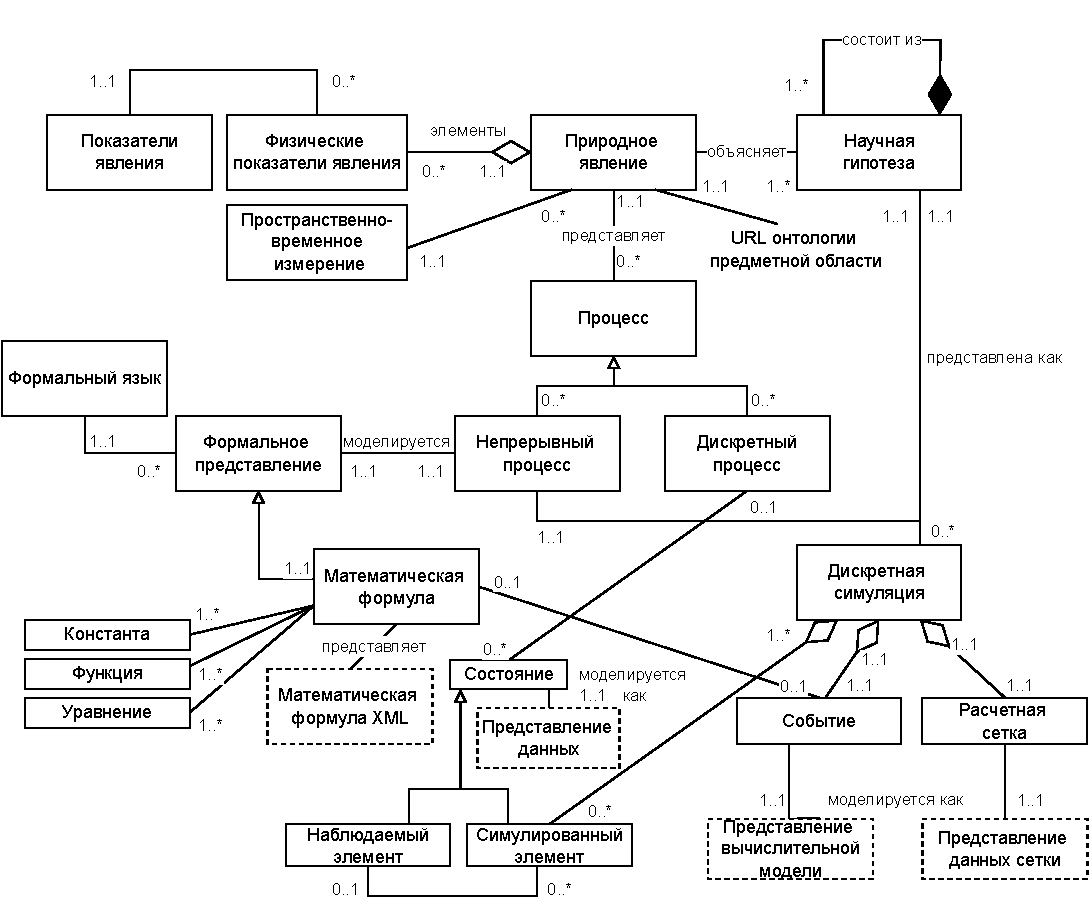
\includegraphics[width=\linewidth]{images/ScHypoConcept}
    \caption{Одна из возможных концептуализаций научной гипотезы.}\label{fig:ScHypoConcept}
\end{figure}

В работе \cite{asgharbeygi2006inductive} представлена математическая формулировка количественных моделей процессов, 
которая обеспечивает формальное кодирование научной моделей в виде системы уравнений, а также неформальное кодирование 
на языке процессов, обозначаемых этими уравнениями. Уточнение модели производится следующим образом. На входе 
необходима изначальная модель; система ограничений, представляющих допустимые изменения начальной модели на языке 
процессов; система базовых (универсальных) процессов, которые могут быть добавлены в начальную модель; наблюдения, 
которым должна соответствовать скорректированная модель. Эти данные обеспечивают эвристический подход, который 
направляет поиск на области пространства модели, которые согласуются с наблюдениями. Алгоритм генерирует множество 
уточненных моделей, которые сортируются по их удаленности от начальной модели и предлагаются вместе со своей 
среднеквадратической ошибкой на тренировочных данных. Расстояние между уточненной и начальной моделью определяется по 
количеству процессов, которые есть в одной, но нет в другой. Состоятельность такого подхода была успешно проверена в 
нескольких областях окружающей среды.

Система формирования гипотез, в основном, однообразна (монотонна) и рассматривается как не вполне подходящая для 
представления знания, в особенности при неполном знании, что часто имеет место в отношении биохимических комплексов. 
В \cite{tran2005knowledge} представлена основанная на знании структура для решения общей задачи формирования гипотез. 
Эта структура была реализована расширением основанной на знании системы <<BioSigNet-RR>>, которая поддерживает 
выработку толерантных представлений и немонотонных логических рассуждений. Главные особенности расширенной системы 
таковы, что они обеспечивают: (1) гладкую интеграцию формирования гипотез с представлением знаний и логическими 
рассуждениями; (2) использование различных ресурсов биологических данных, также как и знаний и опыта человека в целях 
разумной генерации гипотез; (3) поддержку ранжирования гипотез и дизайна экспериментов для проверки гипотез. 
Расширенная система считается прототипом интеллектуального ассистента исследователей – молекулярных биологов.

В проекте «HyBrow» (Hypothesis Space Browser – «Навигатор пространства гипотез») \cite{racunas2004hybrow} гипотезы 
в области биологии представлены как множество предложений исчисления предикатов первого порядка. Если взять сочетание н
абора аксиом, устанавливающих правила, моделирующие известные факты биологии в рамках одной и той же среды, и 
экспериментальные данные, можно обнаружить, что существующая база знаний будет либо противоречить некоторым 
предложениям гипотез, либо подтверждать их, а остальные предложения станут потенциальными открытиями. С получением 
новых экспериментальных данных и формулированием новых правил открытия становятся положительными фактами или 
опровергаются. В случае опровержений должны быть выявлены и удалены из теории, созданной на основе гипотез, те 
правила, которые себя не оправдали. При таком модельно-теоретическом подходе в вопросе подтверждения гипотез 
рассматривается удовлетворение логических импликаций, определенных в модели по отношению к интерпретации. Это может 
быть также применимо к основанным на симуляции исследованиям, где подтверждение выводится из количественного 
анализа "--- сравнения между результатами симуляции и наблюдений \cite{porto2013}. При опровержении или подтверждении 
гипотетических утверждений проект «HyBrow» берет за основу онтологию «OWL» и правила на уровне приложения. 
Проект «HyBrow» обеспечивает разработку гипотез и оценку их на непротиворечивость существующему знанию, а также 
пользуется онтологией гипотез для представления гипотез форме, приемлемой для машин: как отношения между объектами 
(агентами) и процессами \cite{soldatova2011representation}.

Инструмент «HyQue» \cite{callahan2011hyque}, новый этап развития «HyBrow», воспринимает технологии связанных данных 
и использует связанные данные «Bio2RDF», чтобы добавить к «HyBrow» возможности семантической интероперабельности. 
Гипотезы «HyBrow/HyQue» – это предметно-ориентированные утверждения, которые коррелируют с биологическими процессами 
(рассматриваемыми как события) в логике предикатов первого порядка. Гипотезы формулируются как случаи онтологии 
гипотез «HyQue» (HyQue Hypothesis Ontology) и оцениваются с помощью набора вопросов «SPARQL» в сравнении с 
биологически-ориентированными данными «OWL» и «HyBrow». Результаты вопросов оцениваются по некоторой шкале в 
зависимости от того, насколько множество событий соответствует априорным ожиданиям. Оценка по шкале показывает 
уровень поддержки гипотезы данными. Каждое событие оценивается независимо с целью квантифицировать степень поддержки, 
которое оно дает представленной гипотезе. Оценки гипотез привязываются к соответствующим гипотезам как их свойства.

Проект «OBI» (Ontology for Biomedical Investigations – Онтология биомедицинских исследований) 
\cite{brinkman2010modeling} направлен на моделирование дизайна исследования: протоколы, приборы и материалы, 
используемые в ходе экспериментов, а также генерируемые данные. Такие онтологии, как «EXPO» 
\cite{soldatova2006ontology} (см. \cref{fig:EXPO} ) и «OBI», предоставляют возможность документирования всей структуры 
научных исследований: как и с какой целью проведено исследование, какие были сделаны выводы, на какой основе и т.д. 
В результате такой однотипной процедуры по развитию онтологии в работе, заключающейся в получении минимальной 
информации по эксперименту генотипирования (MIGen), рекомендуется использование терминов, определенных в «OBI». 
Использование стандартной или совместимой онтологии для дополнения терминов будет стимулировать междисциплинарный 
доступ к данным и их дальнейшее использование. Для того чтобы сделать исследование более воспроизводимым и допускающим 
повторное использование, предусмотрен сбор возможно большого объема данных.

\begin{figure}[ht]
    \centering
    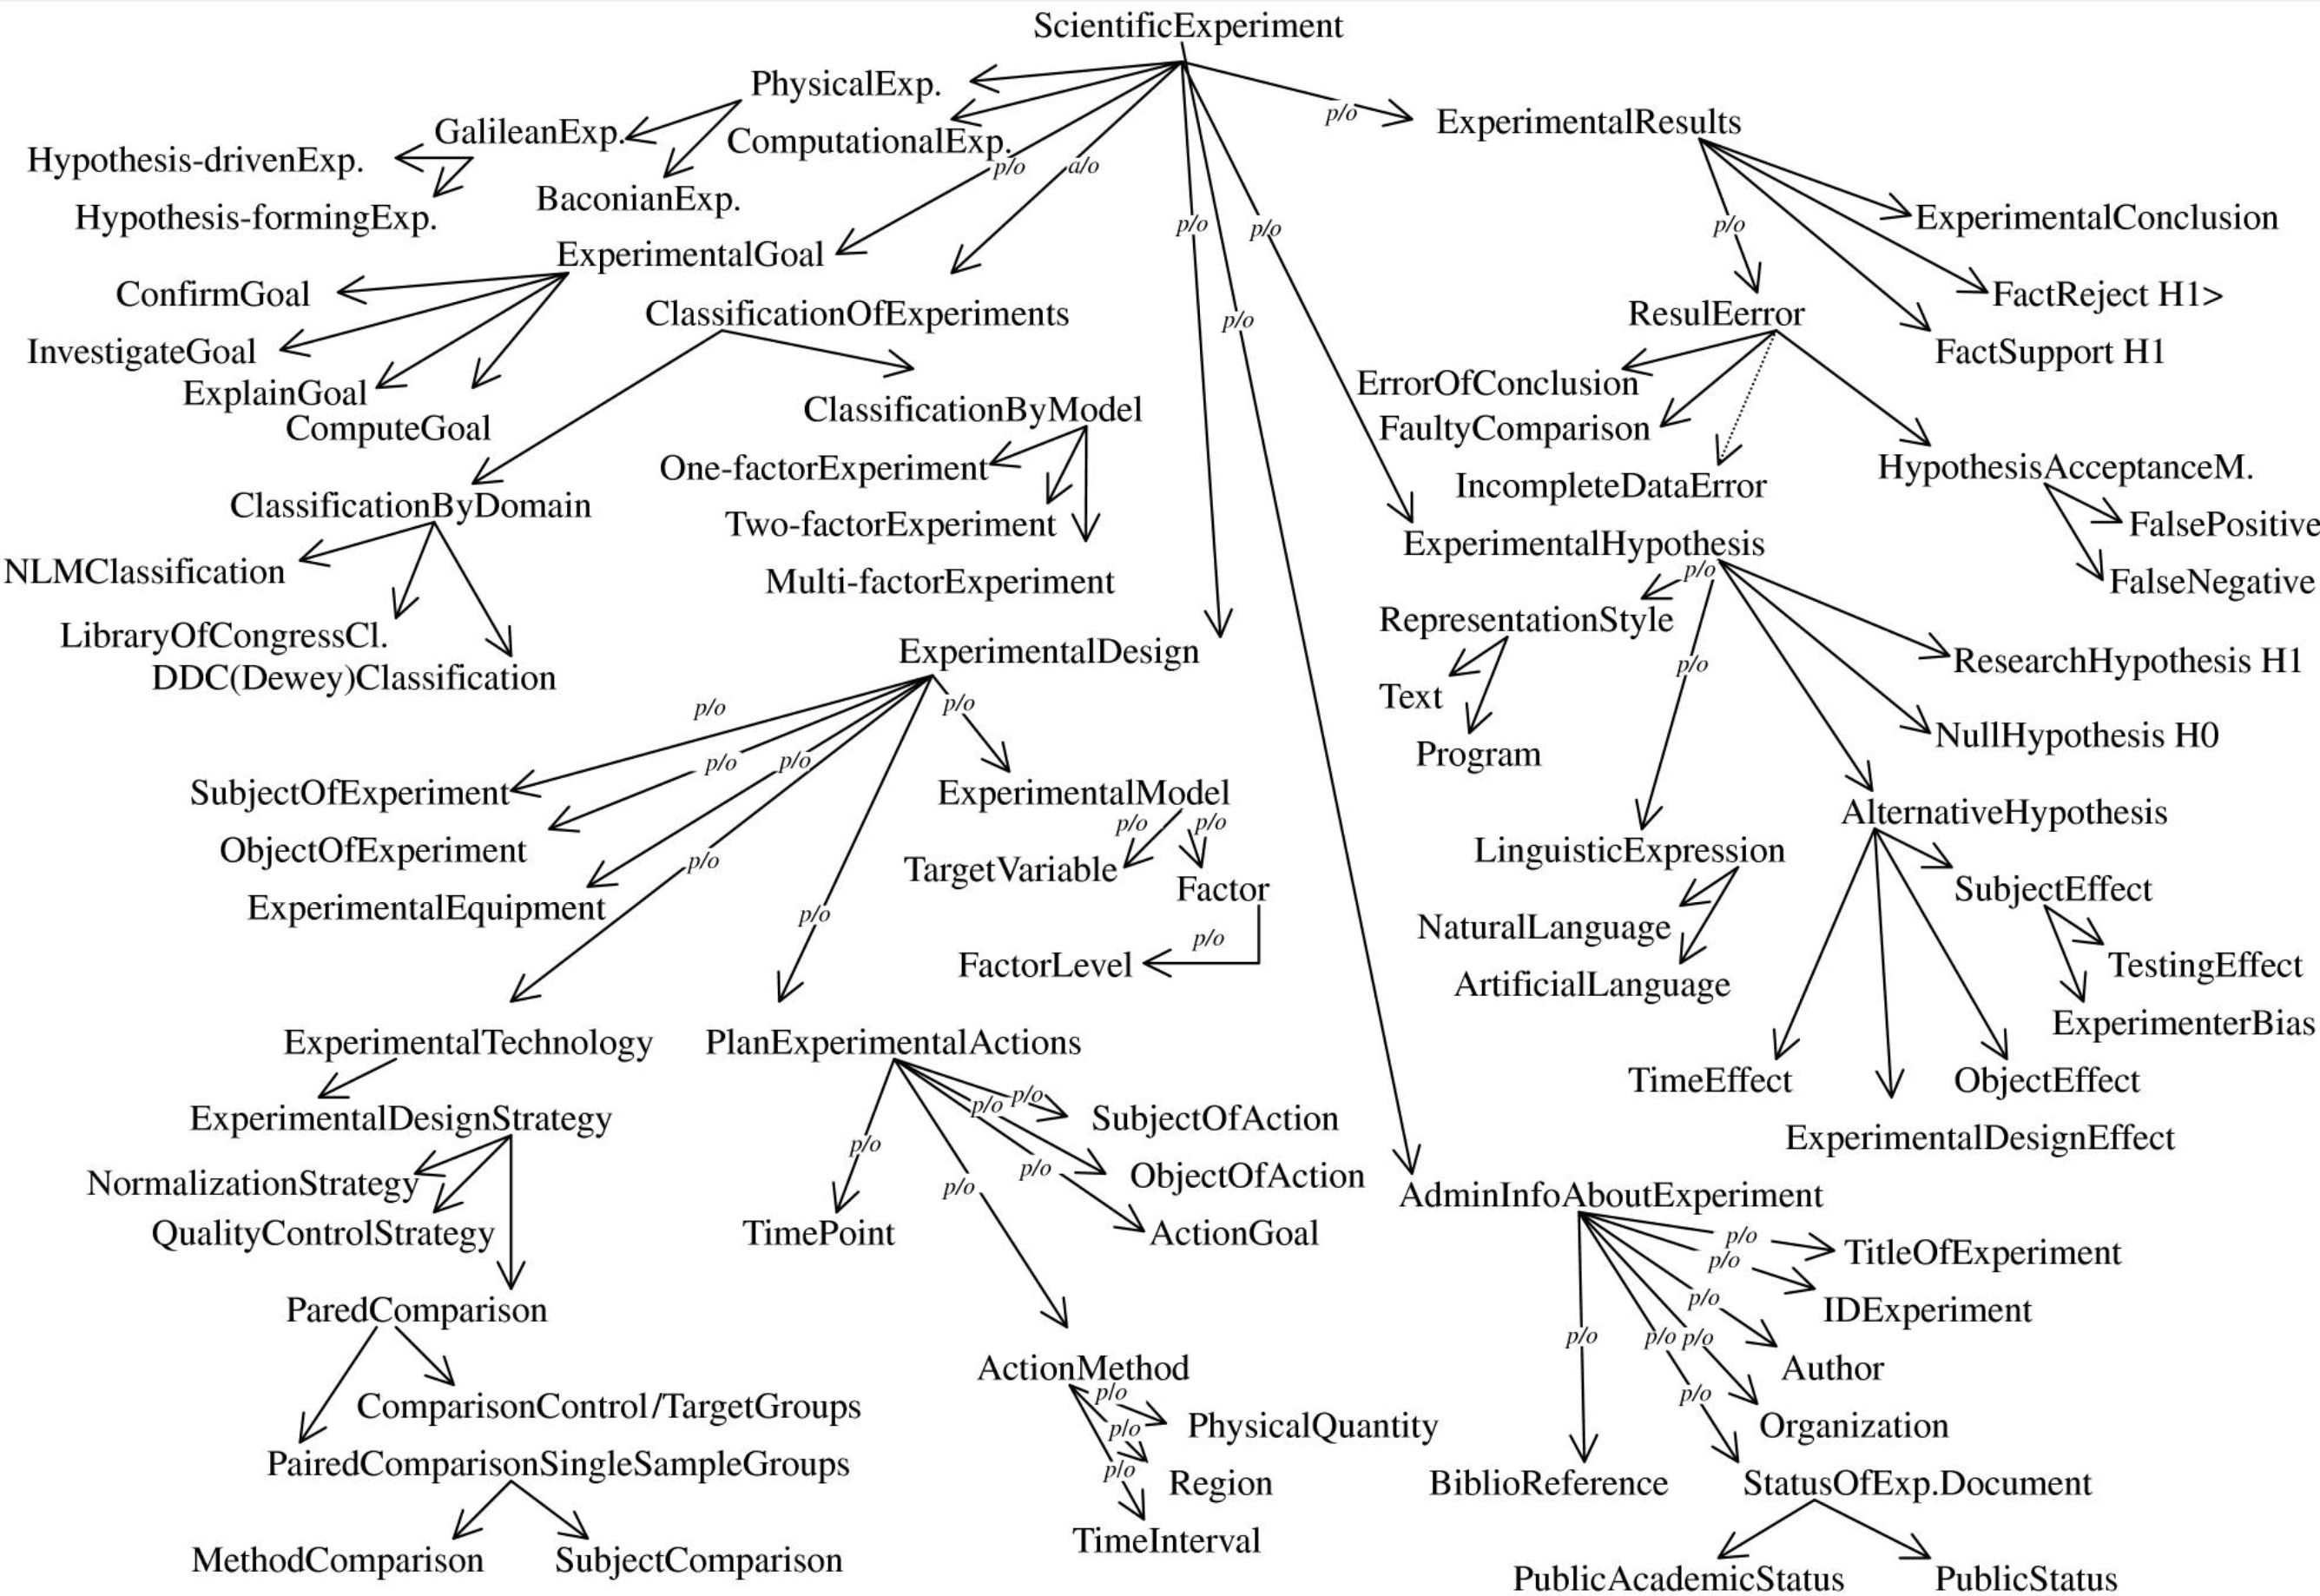
\includegraphics[width=1.0\linewidth]{images/EXPO_onto.png}
    \caption{Фрагмент онтологии научного эксперимента EXPO.}\label{fig:EXPO}
\end{figure}

Моделирование гипотез внедрено в инфраструктуры баз данных, которые развиваются в различных отраслях науки. Один из 
примеров такого рода инфраструктуры имеет наименование «SWAN» (Semantic Web Application in Neuromedicine – 
Семантическое веб-приложение «Нейромедицина») \cite{gao2006swan}. «SWAN» – это проект разработки комплексной 
инфраструктуры знаний для исследовательского сообщества по болезни Альцгеймера. Проект «SWAN» включает в своей 
онтологической модели полный жизненный цикл данных (знаний) в области биомедицинских исследований, в том числе 
организационную поддержку личных данных, генерацию гипотез, ведение экспериментов, организацию лабораторных данных 
и сотрудничество в отношении цифровых препринтов. Общая онтология указывается в «схеме» RDF. Контент проекта «SWAN» 
предназначен для охвата всех этапов процесса «открытия истины» в биомедицинских исследованиях, от формулирования 
вопросов и гипотез, получения экспериментальных данных, совместного с коллегами использования данных, вплоть до полного 
открытия и процесса публикации.

Несколько информационных категорий, которые «SWAN» создает и контролирует определены как подклассы «Утверждения». 
Они включают в себя «Публикацию», «Гипотезу», «Заявку», «Концепцию», «Манускрипт», «Массив данных» и «Аннотацию». 
«Утверждение» может опираться другое «Утверждение» или на любой объект с указанием URL. Например, ученый может 
представить «Комментарий» в отношении «Гипотезы» другого ученого или классифицировать её. Связывание с объектами 
«вне» проекта «SWAN» с помощью URL позволяет использовать информацию «SWAN» в качестве метаданных для организации, 
напр., всех публикаций PDF одного автора, или файлы Excel, в которых зафиксированы данные лаборатории, или все 
веб-сайты инструментов, имеющих отношение к нейробиологии. «Аннотация» может быть как структурированной, так и 
неструктурированной. Структурированность аннотации означает, что она привязана к «Концепции» (с помощью тега или 
термина) к «Утверждению». Неструктурированность аннотации означает привязку свободного текста. 
«Концепции» "--- это узлы вокабуляров, которые также могут быть иерархичными (таксономии).

\section{Основные элементы виртуального эксперимента} \label{sect2_1}

\textit{Определение 1.} \textit{Виртуальный эксперимент} в рамках исследований определяется как 
кортеж $<O, H, M, R, W, C>$, гдe
\begin{itemize}
    \item $O$ "--- это онтология предметной области. Онтология предметной области представляет собой набор понятий и 
            отношений в прикладной области, формально заданных с помощью некоторого языка.
    \item $H$ "--- это набор спецификаций гипотез и взаимосвязей между ними. H является частью онтологии и использует 
            концепции из нее. Вместе они формируют онтологию виртуального эксперимента. Гипотеза "--- это предлагаемое 
            объяснение явления, которое еще предстоит тщательно проверить. 
    \item $M$ "--- это набор моделей. Каждая модель представляет собой набор функций. Каждая модель реализует 
            спецификацию гипотезы. Если модель генерирует ожидаемое поведение какого-либо явления, то говорят, что 
            модель и соответствующая гипотеза подтверждаются наблюдениями.
    \item $R: H \to M$ "--- это отображение из набора гипотез в модели.
    \item $W$ "--- это поток работ. Поток работ представляет собой набор задач, организованных определенными 
            конструкциями (шаблоны рабочего процесса "--- разделение, объединение и т.д.). Каждая задача представляет 
            собой функцию с предопределенной сигнатурой, которая вызывает модели из $M$. Рабочий процесс реализует 
            эксперимент, указывающий, когда следует вызывать каждую модель, соответствующую соответствующим гипотезам. 
    \item $C$ - это конфигурация для каждого запуска эксперимента. Он состоит из полного сопоставления задач 
            рабочего процесса с наборами значений параметров функций.
\end{itemize}

Существует множество возможных реализаций гипотез "--- математические модели, булевы сети, онтологии, предикаты в 
логике первого порядка и т.~д.

Возможными отношениями между гипотезами являются $competes$, который используется для связи конкурирующих гипотез 
и $derived\_by$ для связи двух гипотез, одна из которых использовалась для вывода другой. $derived\_by$ может быть 
использован для формирования решетки гипотез "--- алгебраической структуры с отношением частичного порядка. 
Гипотезы, вытекающие из одной гипотезы, являются атомарными, в противном случае "--- сложными. 
Модель, реализующая гипотезу, должна соответствовать спецификации гипотезы. Если модель генерирует ожидаемое поведение 
какого-либо явления, то говорят, что модель и соответствующая гипотеза подтверждаются наблюдениями.

\section{Жизненный цикл виртуального эксперимента} \label{sect2_2}
Жизненный цикл виртуального эксперимента состоит из четырех этапов и приведен на \cref{fig:lifecycle_ve}. 


\begin{figure}[ht]
    \centering
    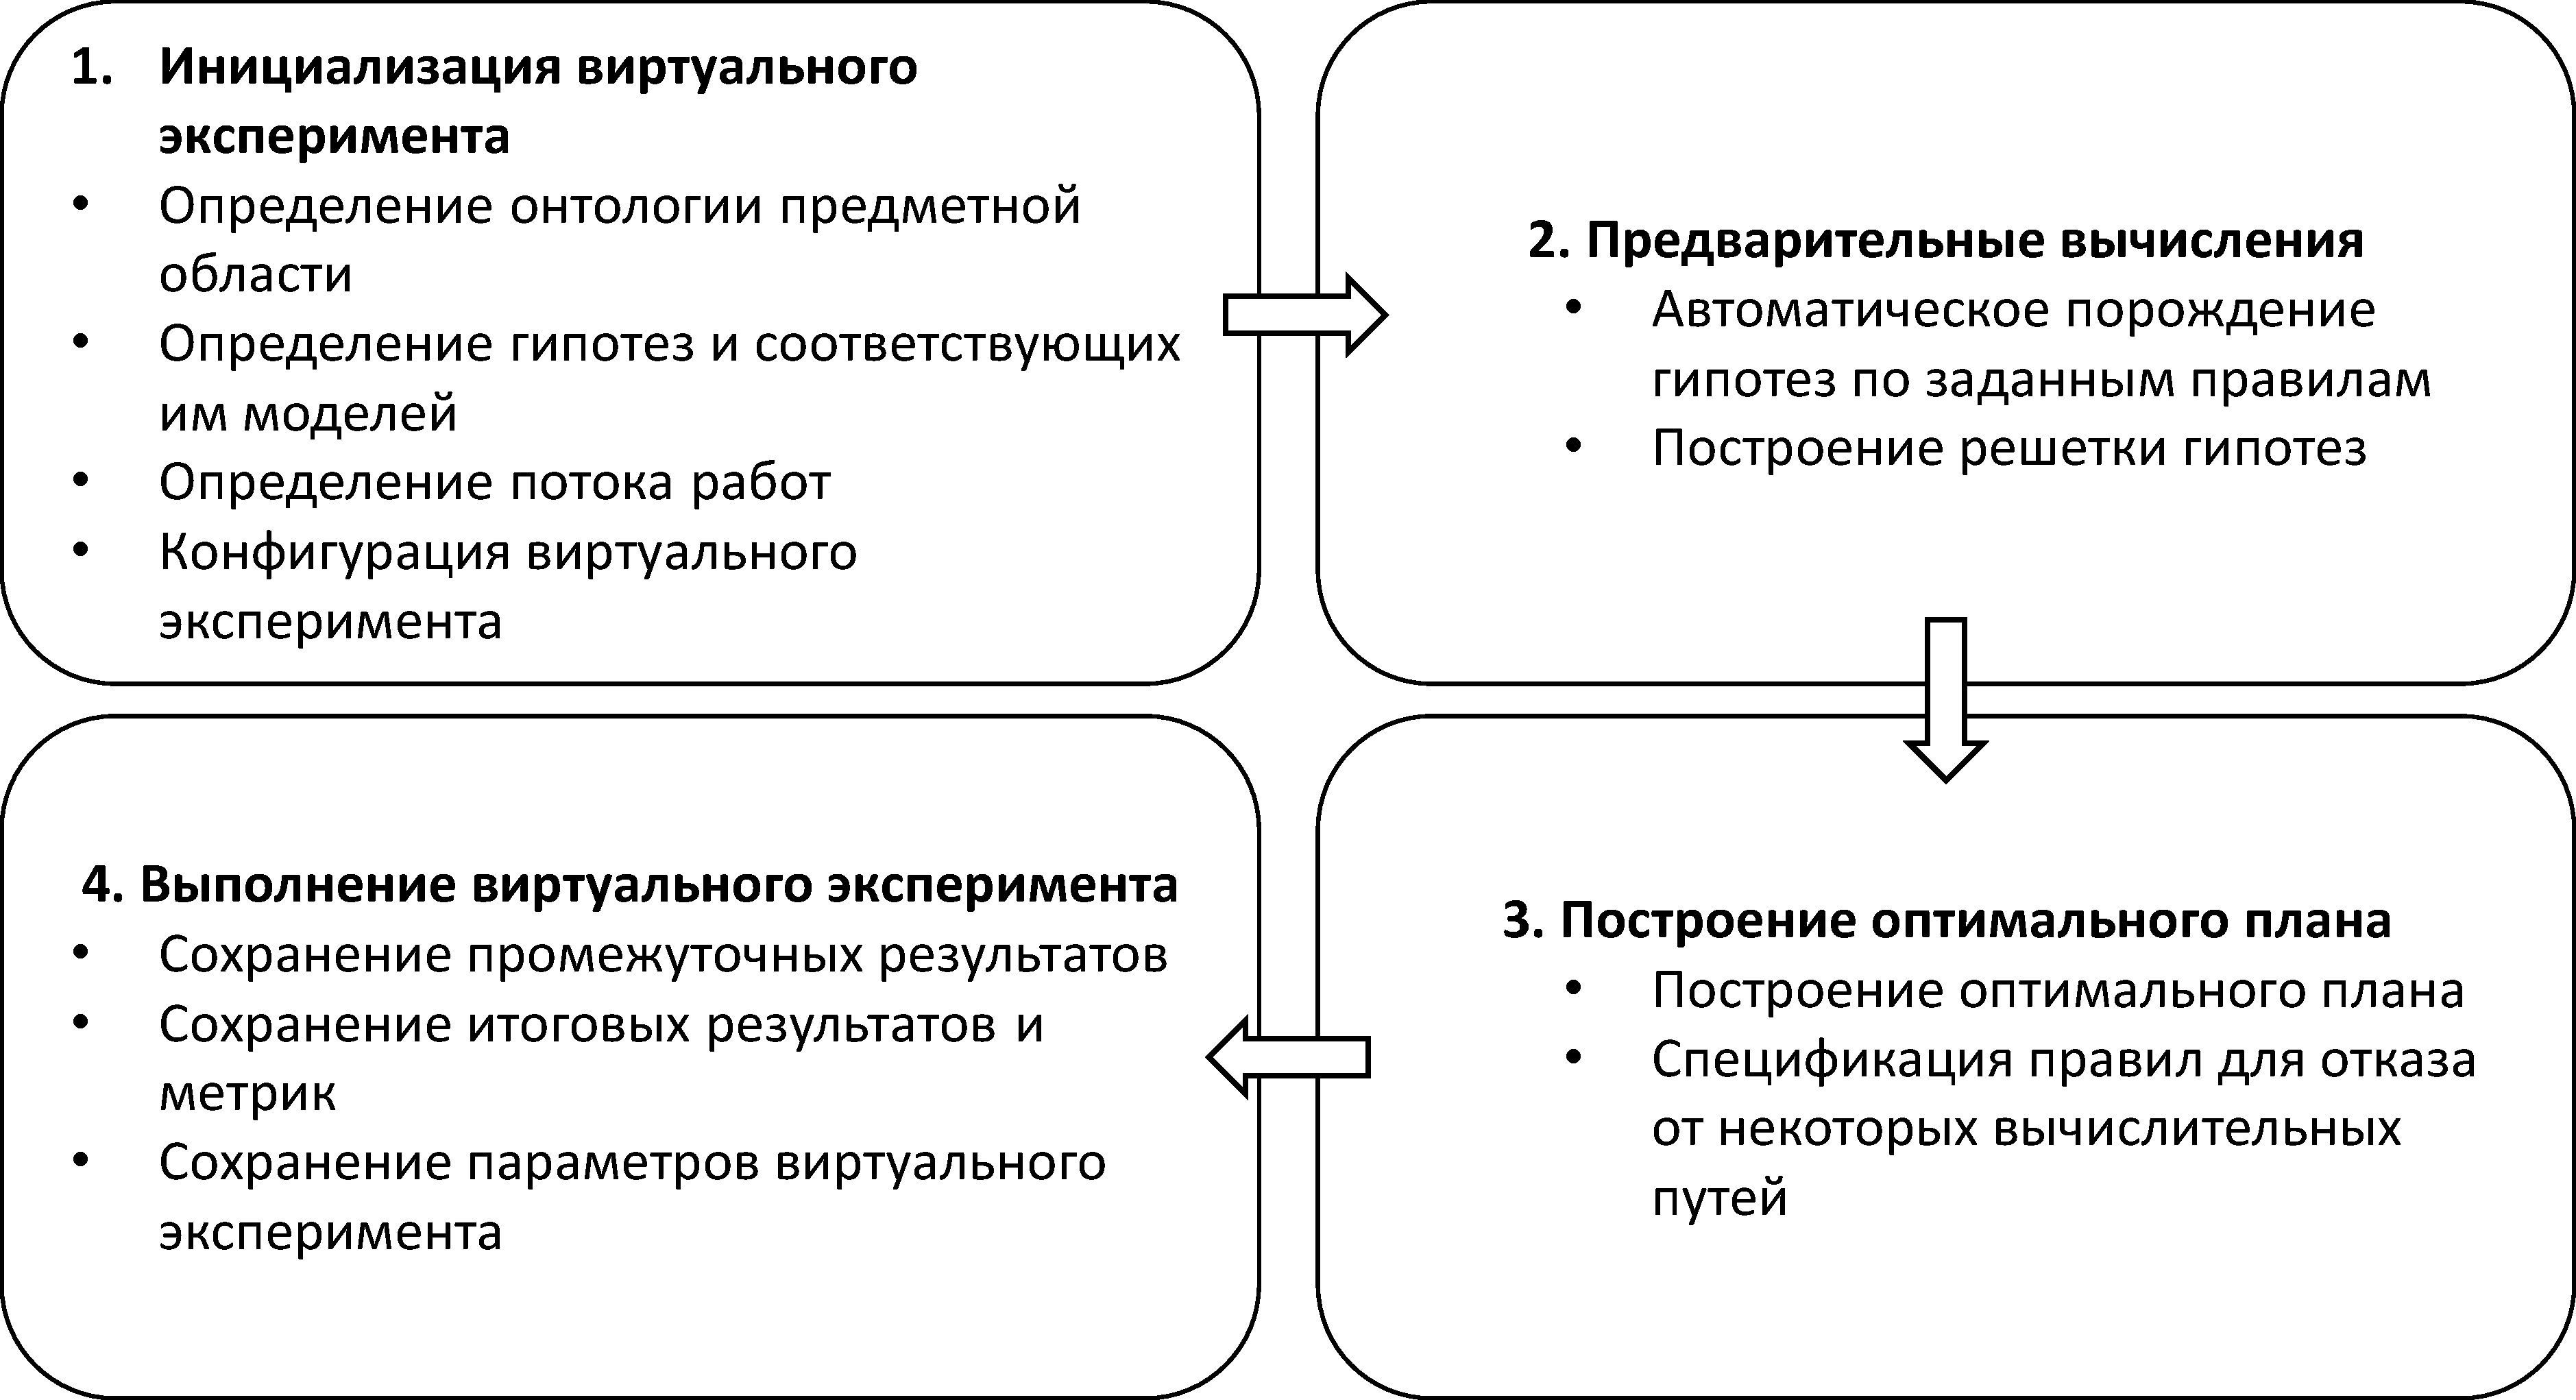
\includegraphics[width=0.9\linewidth]{images/ve_cycle.pdf}
    \caption{Жизненный цикл виртуального эксперимента.}\label{fig:lifecycle_ve}
\end{figure}

На первом этапе происходит инициализация виртуального эксперимента: определение онтологии предметной области, 
определение гипотез и соответствующих им моделей, определение потока работ для исполнения виртуального эксперимента, 
задание конфигурации эксперимента. Поток работ также определяется как направленный ациклический граф. Вершины такого 
графа называются задачами, а каждая задача рассматривается как программа, вызывающая функции, реализующие гипотезы.

На втором этапе по желанию пользователя происходит автоматическое порождение дополнительных гипотез из данных. 
После загрузки виртуального эксперимента в систему происходит автоматическое построение решетки гипотез виртуального 
эксперимента. Используется представление гипотез как специальных структур данных, сочетающих равенства, входящие в 
них переменные и причинно-следственные отображения над ними. Решетка гипотез определяется как направленный ациклический 
граф с вершинами, отвечающими гипотезам. Ребра графа соответствуют отношению завимости между гипотезами, когда 
результат вычислений одной гипотезы используется в вычислениях другой гипотезы. Конструирование решеток отношений 
между гипотезами способствует повышению эффективности управления виртуальными экспериментами, в частности, ускорению 
вычислений с использованием промежуточных результатов, относящихся к независимым гипотезам. 

На третьем этапе происходит построение оптимального плана исполнения нескольких экспериментов. 

На четвертом этапе происходит непосредственное исполнение одного или нескольких виртуальных экспериментов, при этом 
система отслеживает, есть ли в базе данных метаинформации сохраненные результаты исполнения отдельных функций 
эксперимента при заданных параметрах и подставляет их, если совпадение найдено. После исполнения виртуального 
эксперимента результат возвращается эксперту.

По результатам анализа методов манипулирования виртуальными экспериментами был выделен ряд операций для реализации 
в рамках системы по обеспечению полного цикла работы с виртуальным экспериментом. К операциям по работе с виртуальными 
экспериментами, доступным эксперту, относятся добавление, модификация и удаление виртуальных экспериментов, гипотез, 
потоков работ, а также конфигураций экспериментов. Операции, составляющие этап исполнения одного или нескольких 
виртуальных экспериментов, выполняются автоматически для каждой спецификации виртуального эксперимента при ее 
загрузке в систему. 

Промежуточные результаты расчетов, соответствующих вызовам отдельных функций моделей, и оценка их соответствия 
экспериментальным данным сохраняются в базе данных для последующего использования и отслеживания эволюции гипотез и 
моделей виртуального эксперимента.

\section{Решетки гипотез} \label{sect2_3}

Проблема построения структур для одной гипотезы была тщательно изучена в последние годы под разными названиями. 
\noindent Рассматриваются два различных способа нахождения взаимосвязей между гипотезами:
\begin{itemize}
    \item подход <<сверху-вниз>> исходит из анализа математической формы гипотез (обычно в виде набора уравнений);
    \item подход <<снизу-вверх>> исходит из анализа корреляций и зависимостей, присутствующих в данных.
\end{itemize}

Наиболее известным подходом <<сверху-вниз>> является метод, называемый алгоритмом причинного упорядочения 
(COA) \cite{simon1977causal}. Учитывая исследовательскую гипотезу в виде набора математических уравнений, цель 
COA состоит в том, чтобы явно найти отношения асимметрии между переменными уравнений. COA возвращает однозначное 
сопоставление уравнений с переменными для одной исследовательской гипотезы, в то время как взаимодействие нескольких 
гипотез не изучается. Такое отображение определяет ориентированный граф над переменными, где вершины являются 
переменными, а ребра "--- причинно-следственными связями. Переменные, присутствующие в некотором уравнении, 
являются причинно-следственными для зависимой переменной, если в сопоставлении есть запись. 
Сложность COA не учитывается.

В \cite{dash2008note} приводится подробное рассмотрение COA. Авторы формально определяют понятие 
частичного причинного графа и определяют согласованность между ориентированным графом переменных зависимостей 
и частичным причинным графом. Они также вводят основные понятия для выявления причинно-следственных зависимостей, 
скрытых в структуре. Алгоритм возвращает частичное причинно-следственное отображение из разделов набора уравнений 
в разделы одинаковой мощности для набора переменных. Если ровно одно уравнение сопоставляется с одной переменной, 
то сопоставление называется причинным. Показано, что любое действительное полное причинно-следственное отображение 
согласуется с частичным причинно-следственным отображением COA. Вычислительные свойства алгоритмов не обсуждаются. 

Далее в \cite{Goncalves2016} представлен обзор подходов к проблеме причинного упорядочения (COP). COP прямо имеет 
дело со скрытой асимметрией между переменными в заданных наборах математических уравнений. COP исходит из работ по 
моделированию ограничений и рассуждениям \cite{nayak1994causal}. Показано, что COA является NP-трудной проблемой, и 
рекомендуется использовать более эффективный с точки зрения вычислений подход к COP в качестве решения проблемы COA. 
Изображено описание того, как КС связан с проблемой сопоставления гипотез. Вводятся основные определения структур для 
формализации гипотез; представлено предположение о сложности кодирования гипотез из систем уравнений в структуру 
определенного типа. Сложность ограничена $O(|V|*|S|)$, где $S$ "---  структура для набора уравнений $V$ переменных 
с плотностью структуры $S$ (количество появлений переменных) (см. \cref{sect2_3_1} ).

Подход <<снизу-вверх>> реализован в следующих системах: <<Eureqa>> \cite{Schmidt2009}, 
<<Гефест>> (см. \cref{sect1_3_4}), $\Upsilon$-DB (см. \cref{sect1_3_3}).

Eureqa предназначена для вывода символического представления формулы из наблюдений. Авторы демонстрируют, что на основе 
корреляций в наблюдаемых данных отслеживания движения, полученных из различных физических систем, без предварительных 
знаний можно обнаружить законы сохранения геометрии и импульса в виде набора уравнений.

Гефест позволяет проводить виртуальные эксперименты с несколькими конкурирующими гипотезами. Гефест различает два 
разных класса гипотез: введенные исследователем и автоматически выведенные в результате изучения корреляций в данных. 
Все гипотезы сопровождаются вычисленной оценкой точности, например, достигаемым уровнем значимости $p$, исследователю 
показываются только самые высокие оценки для дальнейшей работы. Система не утанавливает взаимосвязи зависимых гипотез 
в виртуальных экспериментах.

В $\Upsilon$-DB предложенный подход дополняет классический статистический подход. Система позволяет работать с двумя 
типами неопределенности "--- теоретической (конкурирующие гипотезы) и эмпирической неопределенностью (альтернативные 
наборы данных). Когда появляются новые данные, этот показатель соответствующим образом корректируется. Моделирование 
обрабатывается как данные, и соответствующие отношения помещаются в ту же базу данных, что и гипотезы. В то же время 
в этих работах не рассматривается вопрос о взаимодействии нескольких гипотез, где доступен рабочий процесс для 
выполнения эксперимента.

\subsection{Построение решетки гипотез} \label{sect2_3_1}
Для определения алгоритма построения решетки гипотез требуются следующие определения из 
\cite{Goncalves2016, kovalev2019constructing}.

\textit{Определение 1.} \textit{Структурой} $S\left(E, V\right)$ называется пара множеств, где $E$ "--- 
это множество уравнений с переменными $V$, так что $|E| \leq |V| $, а так же: 1) в любом подмножестве из $k$ 
уравнений существует не менее $k$ переменных, 2) в любом подмножестве из $k$ уравнений и $r$ 
переменных $\left(k\leq r\right)$, при условии, что значения любых $r-k$ переменных выбираются случайным 
образом, то значения остальных $k$ переменных определяются однозначно.

В данной работе гипотеза $h$ рассматривается как набор уравнений $E_h$ и набор всех переменных $V_h$, указанных 
в $E_h$, так что пара $\left(E_h, V_h\right)$ представляет собой структуру $S\left(E_h, V_h\right)$.

Стоит отметить в определении 1, что структуры состоят из уравнений, а переменные являются их частью только косвенно 
как часть уравнений. Соответственно, все операции множеств, такие как объединение, пересечение и разность, вычисляются 
с использованием уравнений. То есть, если $S(E, V)$ и $S(E',V')$ являются структурами, то $S' \subset S$ , 
когда $E' \subset E$. Определяется дополнительная операция для исключения переменных, т.~е. $T \coloneqq S \div S'$, 
чтобы обозначить структуру $T$, полученную в результате как (1) удаления уравнений $E'$ из $E$, так и 
(2) принудительного исключения переменных $V' = \cup_{f \in E'} Vars(f)$ из $E\setminus	E'$.

\textit{Определение 2.} Пусть $S\left( E, V\right)$ "--- это структура. $S$ является \textit{полной}, если $|E| = |V|$.

\textit{Определение 3.} Пусть $S\left( E, V\right)$ "--- это полная структура. Тогда 
\textit{полное причинно-следственное отображение} над $S$ "--- это биективное отображение $\phi: E\to V$, 
такое что $\forall f \in E$, если $\phi \left( f\right) = x$, то $x \in Vars \left( f \right)$. 
Здесь $Vars \left( f \right)$ "--- это множество всех переменных из уравнений $f \in E$. $|S|$ обозначает число 
появлений переменных в уравнениях, т.~е. $|S\left( E, V\right)| = \sum\limits_{f \in E} Vars\left( f\right)$.


Процедура построения полного причинно-следственного отображения для полной структуры $S\left( E, V\right)$ определена 
в \cite{Goncalves2016}. Вычислительная сложность такого построения ограничена $O\left(|S|*\sqrt{|V|}\right)$.

\textit{Определение 4.} Пусть $S\left( E, V\right)$ "--- это полная структура, где $x_a, x_b \in V$ и $\phi: E \to V$ 
"--- это полное причинно-следственное отображение над $S$. Тогда $C_\phi = \{ \left( x_a, x_b \right) \mid 
\exists f \in E: \phi \left( f \right) = x_b, \text{ } x_a \in Vars\left( f \right) \}$ "--- это множество 
\textit{прямых причинно-следственных зависимостей}. Транзитивное замыкание этого множества обозначается 
$C_\phi^+$ и является набором причинно-следственных зависимостей.  Процедура построения транзитивного замыкания 
для полной структуры $S\left( E, V\right)$ определена в \cite{Goncalves2016}. Вычислительная сложность такого 
построения ограничена $O\left(|S|*|V|\right)$. 

\textit{Определение 5.} Пусть $S\left( E, V\right)$ "--- это структура. Тогда $S$ является \textit{минимальной}, 
если она является полной и нет полной структуры $S'$, такой что $S' \subset S$.

\textit{Определение 6.} Структурная матрица $A_S$ структуры $S\left( E, V\right)$, где $f_1, f_2, \ldots, f_n \in E;
\text{ } x_1, x_2, \ldots, x_m \in V$ "--- это матрица размера $|E| \times |V|$, из нулей и единиц, такая что 
$a_{ij} = 1$, если переменная $x_j \in Vars(f_i)$, иначе~$0$.

\textit{Определение 7.} Решетка гипотез $L$ представляет собой ориентированный ациклический граф, вершины которого 
соответствуют гипотезам с некоторой структурой $S$, а ребра соответствуют отношению $derived\_by$  между гипотезами. 
Отношение $derived\_ by\left(b, a\right)$ означает, что результат вычисления гипотезы $b$ используется при вычислении 
гипотезы $a$.

\textit{Определение 8.} Поток работ $W$ представляет собой ориентированный ациклический граф. Вершины $W$ называются 
задачами. Каждая задача рассматривается как сценарий, вызывающий некоторые функции, реализующие гипотезы. $|W|$ 
обозначает общее количество задач в потоке работ.

Разработанный алгоритм построения решетки гипотез в виртуальных экспериментах представлен в алгоритме
\ref{alg:build_lattice}. На входе алгоритм принимает поток работ $W$ и набор гипотез $H$. 
Если поток работ ссылается на гипотезу, которая не представлена в $H$, алгоритм возвращает ошибку. 
В противном случае возвращается решетка гипотезы $L$.  

Задачи потока работ рассматриваются одна за другой в соответствии с порядком, определяемым направлением ребер. 
Для каждой пары гипотез $h_i, h_j$, где $h_i$ упоминается в текущей задаче, а $h_j$ упоминается в некоторой задаче, 
достижимой из текущей задачи, строится транзитивное замыкание для объединения структур соответствующих гипотез. 
После этого все такие транзитивные замыкания объединяются вместе в $C^+$. Структура результирующей решетки $L$ 
соответствует структуре $C^+$. В качестве вершин $L$ включает гипотезы, в которых встречаются переменные из $C^+$. 
Для каждой пары $\left(x_a, x_b\right)$ в $C^+$ \textit{L} включает ребро 
$derived\_by \left(\phi^{-1}\left(x_b\right), \phi^{-1}\left(x_a\right)\right)$.

\begin{algorithm}
    % \SetKwFunction{isOddNumber}{isOddNumber}
    % \SetKwInput{Input}{Input}
    % \SetKwInput{Output}{Output}
    % \SetKwInOut{KwIn}{Input}
    % \SetKwInOut{KwOut}{Output}


    \KwIn{$W$ "--- \texttt{поток работ}, $H$ "--- \texttt{гипотезы}.}
    \KwOut{$L$ "--- \texttt{решетка гипотез}.}

    \For{$h \in V(W)$}{
        \If{$h \notin H$}{
            \textbf{вернуть} \texttt{'Ошибка: гипотезы не найдены'} 
        }
    }
    
    $ C^+ \gets \varnothing $ 

    $\phi \gets \varnothing $ 

    $L \gets \varnothing $

    $ T \gets V\left(W\right) $

    \For{$t \in T$}{
        $T \gets T \setminus t$

        \For{$h_i \in t$}{
            \For{$remain\_t$ \texttt{в} $T$, \texttt{таких что} $remain\_t$ \texttt{достижим из $t$}}{
                \For{$h_i \in remain\_t$}{
                    $S_i \gets $ \texttt{структура для } $h_i$
                    
                    $S_j \gets $ \texttt{структура для } $h_j$
                    
                    \If{$S_i \cup S_{j}$ "--- \texttt{полная}}{ 
                        \texttt{построить транзитивное замыкание } $C_{ij}^+$ \texttt{для} $S_i \cup S_{j}$
                        $C^+ \gets C^+ \cup C_{i}^+ $
                    }
                }
            }
        }
    }

    $\phi \gets $ \texttt{полное причинно-следственное отображение для} $C^+$
    
    $ L \gets L_{inp}$ 
    \For{\texttt{пара} $\left( x_a, x_b \right) \in C^+$}{
    $ V\left(L\right) \gets V\left(L\right) \cup \{\phi^{-1} \left(x_a\right)\}
             \cup \{\phi^{-1} \left(x_b\right)\}$
    
    $ E \left(L\right) \gets E\left(L\right) \cup \{ derived\_by \left(\phi^{-1} \left(x_b\right), 
    \phi^{-1} \left(x_a\right) \right) \} $
    }

    \KwRet{$L$}
    \caption{Построение решетки гипотез}\label{alg:build_lattice}
\end{algorithm}

\textbf{Лемма 1.} Вычислительная сложность алгоритма построения решетки гипотез для потока работ $W$ и набора гипотез 
$H$ ограничена функцией $ O\left( |W|^2 * |S| * |V| * |H| \right)$, где 
$S = \bigcup\limits_{h \in H} S\left(E_h, V_h \right), V = \bigcup\limits_{h \in H} V_h$.

\textbf{Доказательство.} Самой вычислительно сложной операцией алгоритма является построение транзитивного замыкания. 
Так как алгоритм состоит из трех циклов, то максимальное количество операций транзитивного замыкания не превосходит 
$|W|^2*|H|$, где $|H|$ "--- общее количество гипотез. Сложность построения транзитивного замыкания не превосходит 
$O\left(|S|*|V|\right)$, поэтому вычислительная сложность алгоритма построения решетки гипотез ограничена 
$O\left(|W|^2*|H|*|S|*|V|\right)$.

\textbf{Добавление новой гипотезы.} Алгоритм добавления новой гипотезы в существующую решетку гипотез представлен 
в алгоритме \ref{alg:add_hypothesis}. На входе алгоритм принимает поток работ $W$, существую решетку $L_{inp}$, 
новую гипотезу $H_{add}$. Если поток работ ссылается на гипотезу, которая не представлена в 
$V\left(L_{inp}\right) \cup h_{add}$, алгоритм возвращает ошибку. В противном случае возвращается решетка гипотезы $L$.  

Сначала строится структура $S_{add}$ для добавляемой гипотезы $h_{add}$. Задачи потока работ рассматриваются одна 
за другой в соответствии с порядком, определяемым направлением ребер. Для каждой гипотезы $h_i$, где $h_i$ упоминается 
в текущей задаче, строится соответствующая ей структура. Если объединение этой структуры и структуры $S_{add}$ является 
полным, то строится транзитивное замыкание для объединения структур соответствующих гипотез. После этого все такие 
транзитивные замыкания объединяются вместе в $C^+$. Структура результирующей решетки $L$ соответствует структуре $C^+$. 
В качестве вершин $L$ включает гипотезы, в которых встречаются переменные из $C^+$. Для каждой пары 
$\left(x_a, x_b\right)$ в $C^+$ \textit{L} включает ребро 
$derived\_by \left(\phi^{-1}\left(x_b\right), \phi^{-1}\left(x_a\right)\right)$.

\textbf{Лемма 2.} Вычислительная сложность алгоритма добавления новой гипотезы в существующую решетку гипотез для 
потока работ $W$ и набора гипотез $H$ ограничена функцией $ O\left( |W| * |S| * |V| * |H| \right)$, 
где $S = \bigcup\limits_{h \in H} S\left(E_h, V_h \right), V = \bigcup\limits_{h \in H} V_h$.

\textbf{Доказательство.} Самой вычислительно сложной операцией алгоритма является построение транзитивного замыкания. 
Так как алгоритм состоит из двух циклов, то максимальное количество операций транзитивного замыкания не превосходит 
$|W|*|H|$, где $|H|$ "--- общее количество гипотез. Сложность построения транзитивного замыкания не превосходит 
$O\left(|S|*|V|\right)$, поэтому вычислительная сложность алгоритма построения решетки гипотез ограничена 
$O\left(|W|*|H|*|S|*|V|\right)$.


\begin{algorithm}
    \SetKwFunction{isOddNumber}{isOddNumber}
    % \SetKwInput{Input}{Input}
    % \SetKwInput{Output}{Output}
    % \SetKwInOut{KwIn}{Input}
    % \SetKwInOut{KwOut}{Output}

    \KwIn{$W$ "--- \texttt{поток работ,} $h_{add}$ "--- \texttt{добавляемая гипотеза,} 
        $L_{inp}$ "--- \texttt{существующая решетка гипотез}.}
    \KwOut{$L$ "--- \texttt{решетка гипотез}.}

    \For{$h \in V(W)$}{
        \If{$h \notin V\left( L_{inp}\right) \cup h_{add} $}{
            \textbf{вернуть} \texttt{'Ошибка: гипотезы не найдены'} 
        }
    }
    
    $ C^+ \gets \varnothing $ 

    $\phi \gets \varnothing $ 

    $ T \gets V\left(W\right) $

    $ S_{add} \gets $ \texttt{структура для } $h_{add}$

    \For{$t \in T$}{
        \For{$h_i \in t$}{
            $S_i \gets $ \texttt{структура для } $h_i$
            
            
            \For{$h_i \in remain\_t$}{
                    $S_i \gets $ \texttt{структура для } $h_i$
                    
                    \If{$S_i \cup S_{add}$ "--- \texttt{полная}}{ 
                        \texttt{построить транзитивное замыкание } $C_{i}^+$ \texttt{для} $S_i \cup S_{add}$
                        
                        $C^+ \gets C^+ \cup C_{i}^+ $
                    }
            }
        }
    }

    $\phi \gets $ \texttt{полное причинно-следственное отображение для} $C^+$
    
    $ L \gets L_{inp}$ 
    
    \For{\texttt{пара} $\left( x_a, x_b \right) \in C^+$}{
        $ V\left(L\right) \gets V\left(L\right) \cup \{\phi^{-1} \left(x_a\right)\}
                \cup \{\phi^{-1} \left(x_b\right)\}$
        
        $ E \left(L\right) \gets E\left(L\right) \cup \{ derived\_by \left(\phi^{-1} \left(x_b\right), 
        \phi^{-1} \left(x_a\right) \right) \} $
    }

    \KwRet{$L$}
    \caption{Добавление новой гипотезы в решетку гипотез}\label{alg:add_hypothesis}
\end{algorithm}



\subsection{Решетка гипотез Безансонской модели Галактики}
Различные астрономические модели существенно опираются на гипотезы. Одной из наиболее впечатляющих является 
Безансонская модель Галактики (\textit{BGM}) \cite{czekaj2014besanccon, robin2003synthetic}, которая разрабатывалась 
в течение более чем 35 лет и представляет собой синтетическую популяционную и структурную модель Млечного Пути. 
Она позволяет астрономам выполнять проверку гипотез относительно формирования звезд, их эволюции, а также химической 
и динамической эволюции Галактики. В результате процесса симуляции можно получать следующее: многомерные гистограммы 
внутренних или наблюдаемых характеристик звезд, каталог псевдонаблюдений, или суммарную светимость в заданной 
фотометрической полосе \cite{czekaj2012galaxy}. Изначально целью \textit{BGM} было не только иметь возможность 
симулировать удовлетворительные подсчеты количества звезд, но и глубже тестировать сценарии эволюции Галактики, 
исходя из допущений о скорости звездообразования (\textit{SFR}), начальной функции масс 
(\textit{IMF}) и звездной эволюции.

С моделью связаны явные и неявные гипотезы. Явные гипотезы "--- обычно некоторые системы уравнений, взятые из 
опубликованных исследований и включенные в модель как её составная часть. Часть явных гипотез включены как входные 
элементы модели, напр., скорость образования звезд, начальная функция масс, эволюционные треки, химическая эволюция, 
модели звездных атмосфер, законы распределения плотности звезд, модель межзвездной экстинкции света.

В модель также включены неявные гипотезы. Например, принято, что ни одна популяция звезд Галактики родилась вне 
Галактики. В модель также включены несколько неявных гипотез об образовании диска и допущения относительно темной 
материи. Как правило, перечислить все неявные гипотезы значительно труднее, поскольку многие из них не описаны в 
публикациях, и их сложно распознать, исходя из кода модели.

BGM включает в себя не только большое количество явных и неявных гипотез, но также и сложных отношений между ними. 
Так, некоторые гипотезы независимы, напр., \textit{IMF} и \textit{SFR}, почему и возможно изменять их независимо. 
С другой стороны, некоторые гипотезы связаны между собой, напр., распределение по возрасту, законы распределения 
звездной плотности и потенциала связаны с зависимостью дисперсии скоростей звезд от их возраста через уравнение 
Больцмана и должны согласовываться. Такого рода зависимости сильно усложняют тестирование модели и поддержание 
её в согласованном состоянии, варьируя различные параметры при настройке модели. Другим примером взаимозависимости 
гипотез являются конкурирующие гипотезы.

\textit{BGM} существенно изменилась за прошедшие 30 лет. Этому способствовало появление результатов изучения новых 
данных, новых технологий и развития методов наблюдения. Пример такой эволюции – модель, разработанная в 2014 г., 
если сравнить её с предыдущими версиями, работает с вариантами \textit{SFR}, \textit{IMF}, эволюционными треками 
и атмосферными моделями. Эти гипотезы вводятся как входные параметры модели, поэтому пользователь может их 
варьировать. Второе усложнение модели – введение двойных звёзд: значительное изменение, поскольку двойные системы 
звёзд составляют примерно 50\% общего наполнения Млечного Пути. Авторы новой версии подчеркивают важность 
понимания взаимозависимости различных гипотез и необходимость инструментов эволюции модели: В практическом плане, 
чтобы построить Галактику из базовых составляющих, нам пришлось реконструировать предыдущую модель и внести 
существенные изменения в построение кода. Это требовало хорошего понимания лежащих в основе отношений между 
всеми предусмотренными компонентами \cite{czekaj2012galaxy}. 
    
В дальнейшем планируется сосредоточиться на обновленной \textit{BGM} \cite{czekaj2014besanccon}, в которой авторы 
привлекают внимание к изучению тонкого диска Галактики и используют Tycho-2 как тестовый набор данных. Набор данных 
Tycho-2 и статистический тест типа $\chi^2$ используются для проверки различных версий этих гипотез, с тем чтобы 
выбирать наиболее пригодные и обновлять модель для лучшего соответствия предоставленным данным. 
Тесты выполнялись путем сравнения количества звезд и цветовых распределений $(B-V)T$ между данными и результатами 
симуляций. Два разных теста были использованы для оценки глобальной соразмерности звездных плотностей и проверки 
формы цветового распределения. 

Другие параметры, которые будут подвергнуты проверке: количества звезд, скорость распространения радиоволн, звездные 
величины, цвета звезд, их собственное движение, параллакс, эффективные температуры, сила тяжести и металличность. 
Авторы используют гистограммы, два критерия согласия (максимальная вероятность и тест $\chi^2$), а также критерии 
Колмогорова---Смирнова и Андерсона---Дарлинга для параметра скорости. 

Параметры одной гипотезы могут быть связаны друг с другом непосредственно с помощью уравнений. Существуют также 
косвенные связи параметров нескольких гипотез, например, параметр \textit{SFR} коррелирует с наклонами \textit{IMF}. 
Это подразумевает, что нельзя было бы дать наилучшее решение для конкретной переменной, не соотнеся ее с другими. 
Таким образом, существует необходимость в поддержке поиска корреляции между гипотезами

Пользователю разрешается изменять не все ингредиенты модели. Это делается потому, что если какая-то гипотеза 
изменяется в модели и никакие дальнейшие корректировки для зависимых гипотез не вносятся, согласованность модели 
нарушается. Кроме того, модель обладает свойством быть самосогласованной, что означает, что при изменении входных 
значений, если это возможно, гипотезы, полученные с помощью измененной, должным образом корректируются, чтобы не 
нарушать фундаментальные уравнения астрономии. Следовательно, производное по отношению должно быть смоделировано. 
Кроме того, системный компонент должен обеспечивать возможность корректировки и калибровки любой гипотезы, 
доступной в модели.

Поскольку количество экспериментов огромно из-за увеличения размера семейства конкурирующих гипотез, теперь не все 
возможные проверяются на всем небе. Изучение способов сокращения количества экспериментов, которые дают наилучшую 
подгонку, и выбора того, когда и если отказаться от дальнейших вычислений эксперимента, является основной частью 
требований к новой системе. Использование информации из эксперимента, проведенного как локально, так и другими 
исследовательскими группами, может быть полезным в достижении этой цели.

В некоторых исследованиях анализа с интенсивным использованием данных подчеркивается роль полос ошибок. Поскольку 
данные в астрономии обычно предоставляются с ошибками, \textit{BGM} использует специальные методы для работы с 
таким типом неопределенности. Компонент, поддерживающий статистические инструменты, который работает с индикаторами 
ошибок, является основным требованием к инфраструктуре

Поскольку некоторые составляющие модели находятся в тесной взаимосвязи (такие как IMF, SFR и локальная плотность 
массы), авторы определили конфигурацию модели по умолчанию как сочетание нового набора составляющих, которые 
существенно улучшают согласие с данными Тихо. Поток работ используется для реализации эксперимента \textit{BGM}, 
определяющего, когда следует вызывать каждую модель, которая соответствует связанным гипотезам. Поток работ также 
претерпел изменения по сравнению с первой версией, например, для обработки тонких дисков введены новые действия, 
зависящие от гипотез \textit{IMF} и \textit{SFR}. Это развитие можно отследить только с помощью публикаций. 


Так, были подвергнуты проверке 11 функций IMF, 2 функции SFR, 2 набора эволюционных треков, 3 набора атмосферных 
моделей, 3 значения возраста формирования тонкого диска, 3 набора значений плотности массы звездного объема 
тонкого диска. Пример гипотез для \textit{SFR} приведен на \cref{fig:SFR}.

\begin{figure}[ht]
    \centering
    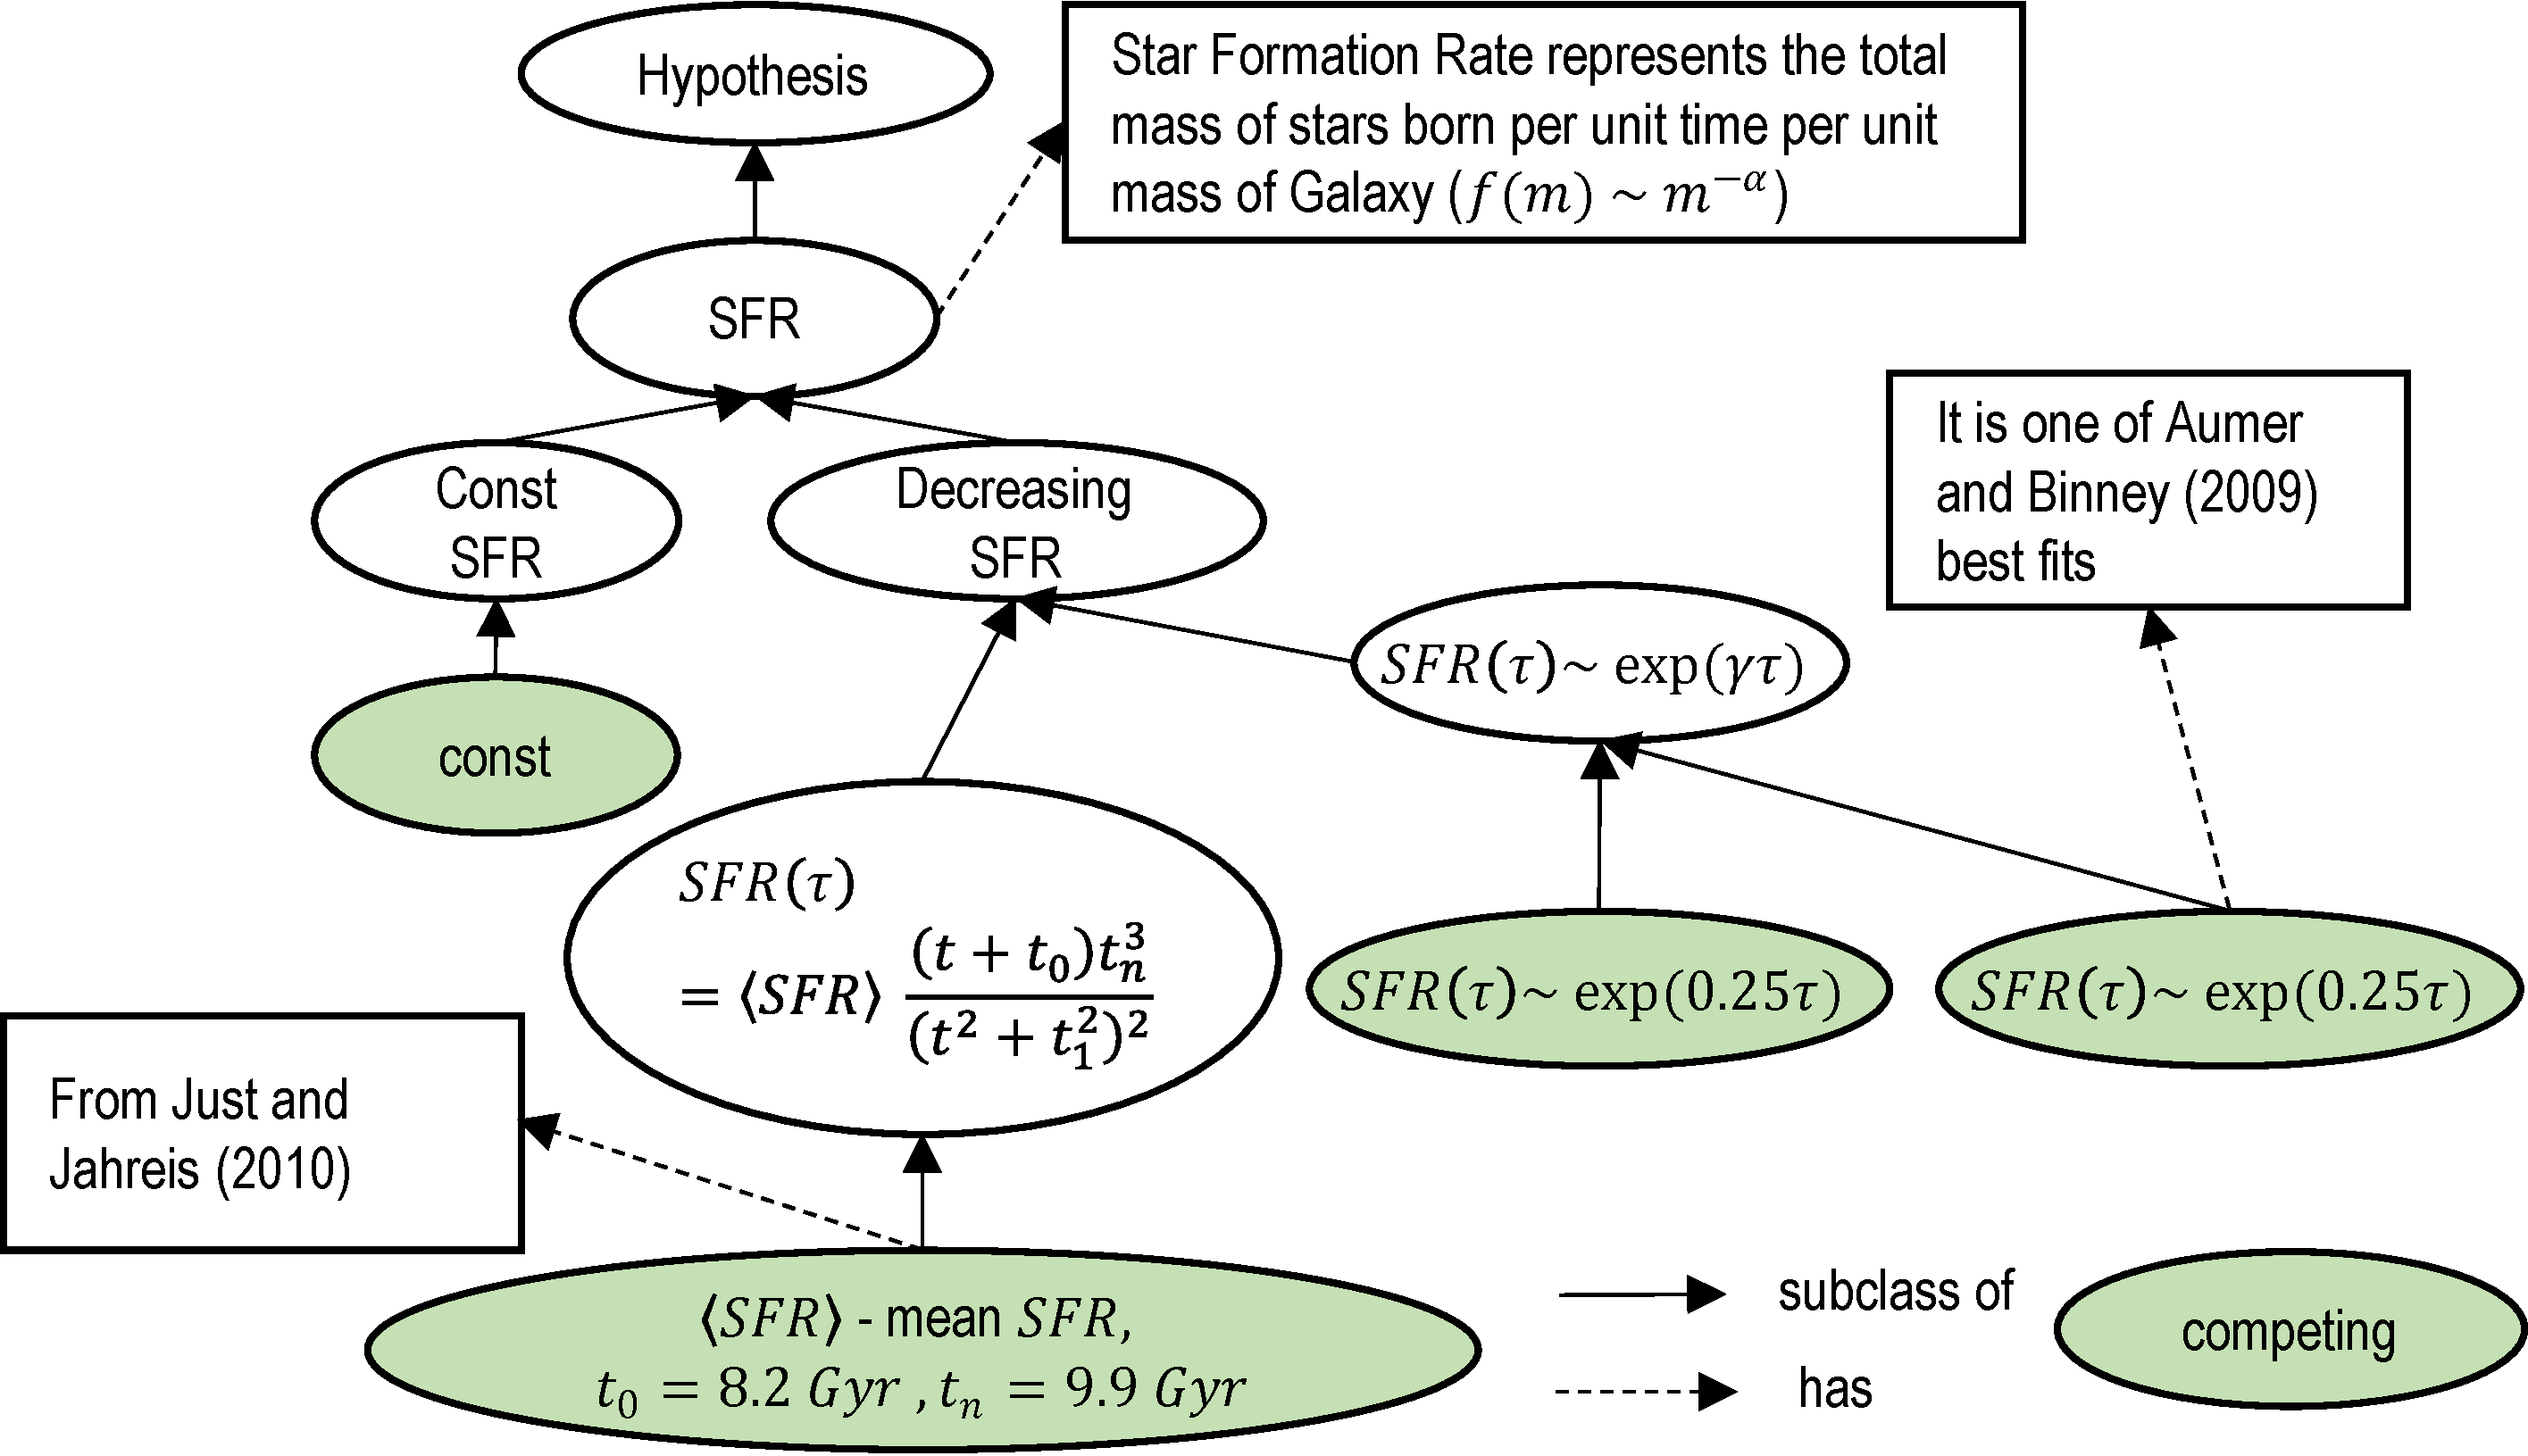
\includegraphics[width=1.0\linewidth]{images/SFR.pdf}
    \caption{Гипотеза SFR для BGM.}\label{fig:SFR}
\end{figure}

\textit{SFR} определяется для семи возрастных ячеек Тонкого диска (структурного компонента Галактики) следующим образом:

\begin{equation}
    SFR(i) = exp(\gamma \times x_c(i)) \times d
\end{equation}

где $x_c(i)$ "--- возраст в центре ячейки $i$, а $d$ "--- размер этой ячейки. Различными значениями 
$\gamma = \{0.12, 0.25\}$ определяются две конкурирующие гипотезы.

IMF определяется следующим образом:
\begin{equation}
    IMF(m) = m^{-\alpha}
\end{equation}

где $\alpha$ "--- это варьируемый параметр. По мере развития модели в модель вводятся новые значения параметра, 
например, в настоящее время существует 11 различных вариантов для \textit{IMF}.

Локальная объемная плотность $\rho(i)$ "--- это гипотеза для коэффициента нормализации, необходимого для вычисления 
функции звездной рождаемости. Он вычисляется для каждого $i$ на основе предопределенных 
законов плотности и \textit{SFR}.

Функции звездной рождаемости определяются с использованием уравнения:
\begin{equation}
b(m, t)dm dt \approx f\left(SFR\left(i\right), \rho\left(i, SFR\left(i\right)\right)\right) 
\times IMF(m)\Delta m \Delta i
\end{equation}

Стоит отметить, что модель определения массы включает в себя и другие гипотезы 
(полный список гипотез показан на \cref{fig:BGM_lattice}).

В качестве примера мы рассмотрим часть потока работ, которая состоит всего из 
трех последовательных задач (см. \cref{fig:BGM_workflow}). 


\begin{figure}[h!]
    \centering
    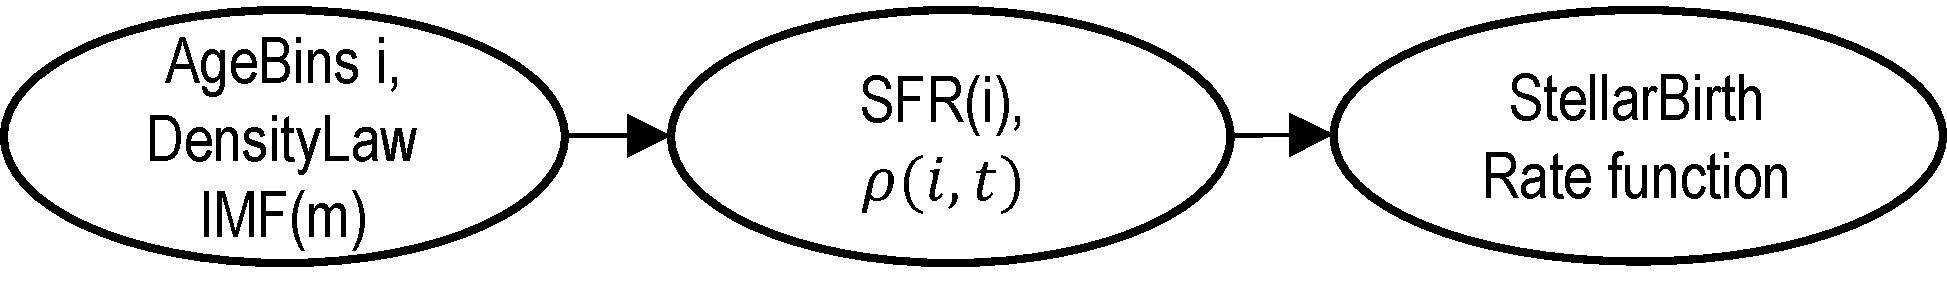
\includegraphics[width=0.7\linewidth]{images/BGM_workflow.pdf}
    \caption{Поток работ для модели определения массы, каждая задача выполняется 
            в соответствии с определенными гипотезами.}\label{fig:BGM_workflow}
\end{figure}

\begin{figure}[ht]
    \centering
    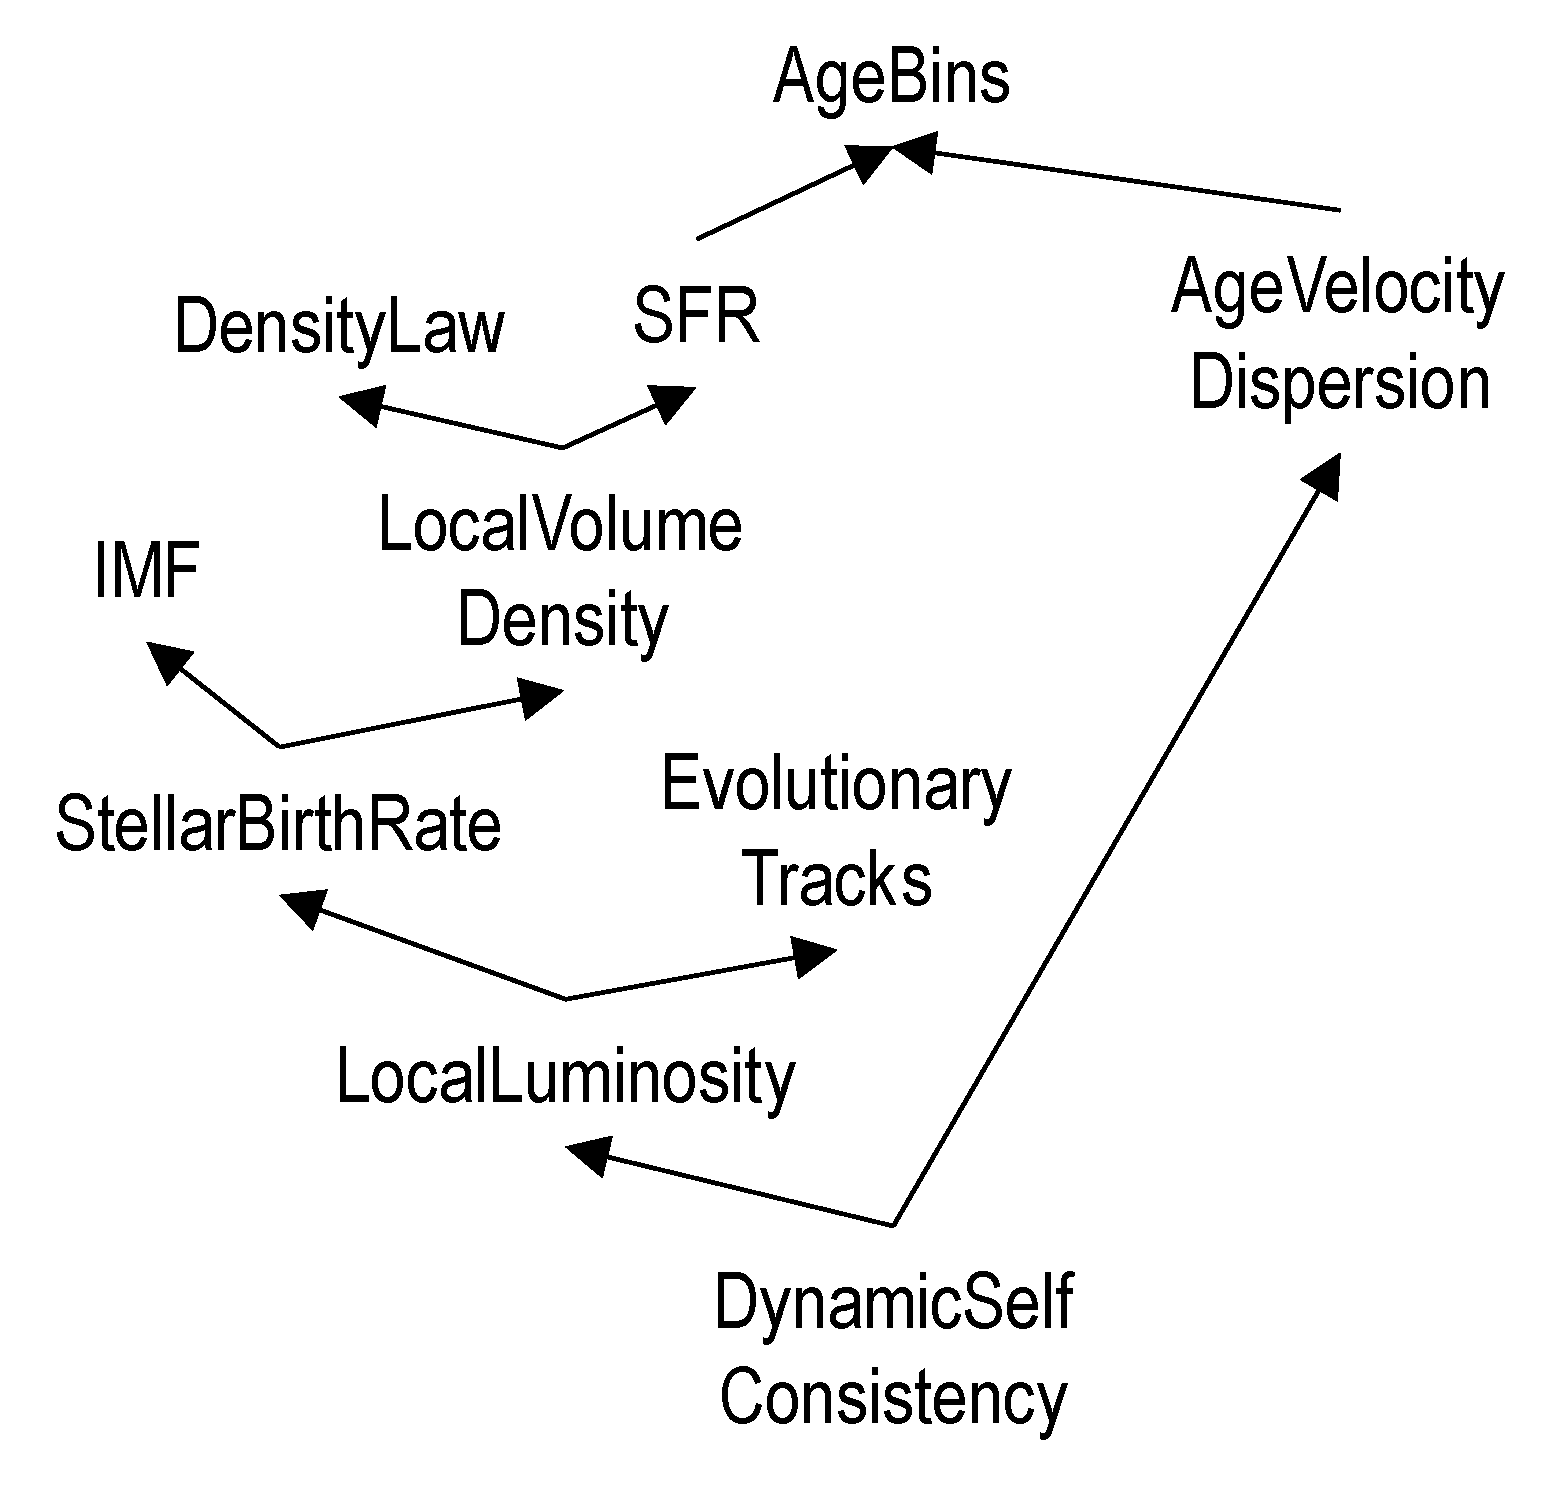
\includegraphics[width=0.6\linewidth]{images/BGM_lattice.pdf}
    \caption{Решетка гипотез  для определения массовой модели с отношением \textit{derived\_by}.}\label{fig:BGM_lattice}
\end{figure}

Первая задача включает гипотезы, соответствующие возрастным ячейкам гипотез, законам плотности и \textit{IMF(m)}. 
Вторая задача состоит из гипотез, соответствующих гипотезам \textit{SFR(i)} и локальной объемной плотности 
$\rho(i, t)$. Третья задача соответствует гипотезе о функции звездной рождаемости.

В соответствии с алгоритмом \ref{alg:build_lattice} строятся структуры для различных пар гипотез. Например, структура 
объединения для возрастных ячеек гипотез и $\rho(i, t)$ является неполной, а структура объединения для возрастных 
ячеек гипотез и $SFR(i)$ является полной. Транзитивное замыкание для возрастных ячеек и $SFR(i)$ 
равно $\{(i, x_c(i)); (i, d)\}$. Транзитивное замыкание индуцирует две вершины \textit{(AgeBins, SFR)} 
и одно ребро \textit{(derived\textunderscore by(AgeBins, SFR))} решетки. Результирующая решетка гипотез 
для модели определения массы изображена на \cref{fig:BGM_lattice}.

Построив решетку гипотез в виртуальном эксперименте, становится возможным формально анализировать и повторно 
использовать результаты частичных вычислений в виртуальном эксперименте. Например, если изменяется только 
гипотеза \textit{IMF}, нет необходимости в повторном вычислении \textit{SFR} или функции локальной объемной плотности.

Разработана концептуальная спецификация виртуального эксперимента для определения модели масс в БГМ, в том 
числе онтология основных понятий предметной области (галактика, тонкий диск, толстый диск, гало, звезда, 
популяция звезд) и спецификации основных гипотез (с использованием языка OWL) и поток работ, формализующий 
виртуальный эксперимент.

На основании анализа предметной области моделирования Галактики (статей, посвященных БГМ и программного 
кода реализации БГМ на языке Фортран 77) выделены основные гипотезы, составляющие модель, например, 
начальная функция масс (IMF) и функция скорости образования звезд (SFR). Начальная функция масс представляет 
собой распределение массы данной популяции звезд и представляется стандартным степенным законом. 
В БГМ функция представлена кусочной функцией с 2 или 3 частями. Существуют ограничения на доступное 
отношение массы к массе Солнца. Представлено 10 различных версий гипотезы, 4 из них являются 2-кусочными 
функциями и 6 из них 3-кусочными.

Определен поток работ виртуального эксперимента, включающий следующие задачи: расчет распределения объемной 
плотности звезд в Галактике (при этом звезды делятся на 7 основных возрастных популяций, для каждой из 
популяций вычисляются параметры распределения), расчет распределения поверхностной плотности звезд для каждой 
популяции, взаимная корректировка объемной и поверхностной плотностей, моделирование параметров звезд 
(например, массы) для каждой из популяций, разбиение звезд на живые звезды и остатки (возможные звёзды, для 
которых возрастное и массовое сочетание противоречат друг другу), пересчет звездного состава тонкого диска с 
использованием уравнения Пуассона, численное решение уравнение Больцмана для популяций звезд с целью проверки 
соответствия модели основным физическим законам.

По представленному потоку работ и гипотезам построена решетка зависимости гипотез с использованием реализованного 
алгоритма. Так, например, гипотеза о рождении новых звезд является зависимой от IMF и косвенно 
от SFR через гипотезу о локальной объемной плотности.

Применяется процедура построения зависимости значения поглощения света в межзвёздной среде от расстояния 
(d) до звезды с определёнными галактическими координатами $(l, b)$ на основе данных многоцветной фотометрии. 
Моделируется наблюдаемый блеск ($m$) в зависимости от спектрального типа звезды ($SpT$), расстояния до неё ($d$) 
и значения межзвездного поглощения ($A_i$) для каждого фотометрического диапазона ($i$). На основе сравнения с 
реальной наблюдаемой яркостью выбирается наиболее подходящий набор моделируемых параметров. Модель позволяет 
получать с приемлемой точностью астрофизические параметры: эффективную температуру, гравитацию, металличность, 
визуальное поглощение и отношение полного поглощения к селективному. Результаты оценки поглощения в заданном 
направлении могут использоваться для выбора адекватной непротиворечивой модели параметров соседних звёзд.



\section{Непротиворечивость виртуального эксперимента}\label{sect2_5}
Для корректного запуска виртуальный эксперимент должен быть \textit{непротиворечивым}. 
Для этого должны выполняться следующие условия:
\begin{enumerate}
    \item Должны быть опредены все элементы виртуального эксперимента $O, H, M, R, W, C$.
    \item Число гипотез должно быть не менее числа задач в потоке работ $|H| \geq |V(W)| $.
    \item Число моделей должно быть не менее числа гипотез $|M| \geq |H|$.
    \item Для каждой гипотезы должна быть опредена реализующая ее модель: $ \forall h \in H: \exists m \in M$ такой, 
            что $h \rightarrow m \in R$.
    
    \item Для каждой задачи потока работ должен существовать набор значений параметров вызываемых функций 
            $ \forall t \in V(W): \exists c \in C$.
    \item После построения решетки гипотез запускается алгоритм \ref{alg:consistence} проверки отсутствия 
            некорректных зависимостей гипотез в потоке работ.
\end{enumerate}

Если нарушено условие 1), то платформа не сможет запустить выполнение виртуального эксперимента.
При нарушении условия 2) у некоторых задач потока работ будут отсутствовать соответствующие им гипотезы, что не 
позволит корректно построить решетку гипотез. При нарушении условия 3) и 4) некоторым гипотезам не будут 
сопоставлены модели, следовательно их будут невозможно исполнить. Условие 5) гарантирует, что для каждой модели 
существуют параметры ее запуска. Условие 6) необходимо для избежания циклов в графе потока работ, что приведет к 
некорректному построению решетки гипотез. Если гипотеза используется в задаче потока работ, то она не может быть 
использована в других задач, достижимых из этой. 

\begin{algorithm}
    \SetKwFunction{isOddNumber}{isOddNumber}
    % \SetKwInput{Input}{Input}
    % \SetKwInput{Output}{Output}
    % \SetKwInOut{KwIn}{Input}
    % \SetKwInOut{KwOut}{Output}

    \KwIn{$W$ "--- \texttt{поток работ}, $L_{inp}$ "--- \texttt{решетка гипотез}.}
    \KwOut{\textit{True} "--- \texttt{некорректные зависимости отсутствуют,} \textit{False} "--- \texttt{иначе}.}

    \textit{correct} $\gets$ \textit{True}

    \For{$t \in V(W)$}{  \Comment{задачи перебираются последовательно}

        \For{$h \in t$}{\Comment{проверяются все гипотезы из задачи}
            \texttt{найти все зависимые $\{h_d\} \in V(L_{inp})$ от $h$ }
            
            \For{\texttt{$remaining\_task$ достижимых из $t$}}{

                \If{$\{h_d\} \cap H_t \neq \emptyset\  \alpha\  s.t.\  H_t \in remaining\_task$}{
                    \Comment{Эксперимент определен некорректно}

                    correct $\gets$ \textit{False}   
                }
            }
        }
    }
    \KwRet{correct}
    \caption{Проверка отсутствия некорректных зависимостей гипотез в потоке работ}\label{alg:consistence}
\end{algorithm}


В алгоритме \ref{alg:consistence} для каждой из задач, которые перебираются последовательно, проверяется, что все гипотезы из 
данной задачи не имеют пересечения зависимых от них гипотез с гипотезами с гипотезами из достижимых задач для данной 
задачи. При нарушении этого условия, возвращается, что эксперимент построен некорректно.

При нарушении любого из этих свойств возвращается ошибка определения виртуального эсперимента.

\section{Планирование выполнения виртуального эксперимента}\label{sect2_}
В алгоритме \ref{alg:plan} представлено построение плана виртуального эксперимента. На вход алгоритм принимает 
конфигурацию эксперимента, решетку гипотез, а на выходе возвращает два набора гипотез, модели для которых требуют или 
не требуют пересчета.



\begin{algorithm}
    \SetKwFunction{isOddNumber}{isOddNumber}
    % \SetKwInput{Input}{Input}
    % \SetKwInput{Output}{Output}
    % \SetKwInOut{KwIn}{Input}
    % \SetKwInOut{KwOut}{Output}

    \KwIn{$C$ "--- \texttt{конфигурация эксперимента}, $L$ "--- \texttt{решетка гипотез}.}
    \KwOut{$P_{ne}$ "--- \texttt{множество гипотез, для которых требуется пересчитать модели}, 
           $P_{e}$ "--- \texttt{прочие.}}

    $L_{n} \gets $ ближайшая для $L$ решетка в репозитории данных

    $P_{ne} \gets \varnothing , P_{e} \gets \varnothing $ 

    $F \gets \varnothing $

    $V \gets V(L_n)$

    % DFS 
    \For{$h \in V$}{ \Comment{начало с самой верхней гипотезы}
        \If{$\forall c_m \in C, \forall m \in M \  \alpha \  s.t.\  \nexists h \to m(c_m)$}{
            \Comment{в репозитории нет вычисленной части эксперимента}
            $H_{dep} \gets $ все зависимые гипотезы от $h$
            
            $P_{ne} \gets P_{ne}  \cup H_{dep} \cup h$

            $F \gets F \cup H_{dep} \cup h$
        }
        \Else{
            \Comment{в репозитории есть вычисленный фрагмент}

            $P_{e} \gets P_{e} \cup h$

            $F \gets F \cup h$
        }
        
        $V \gets V \setminus F $
    }
        
    \KwRet{$P_{ne}, P_{e}$}
    \caption{Построение плана виртуального эксперимента}\label{alg:plan}
\end{algorithm}

Сначала ищется ближайщая решетка, которая уже была вычисленна. После этого происходит поиск в глубину, начиная с 
гипотезы, у которой нет входных ребер. Если для всех параметров из конфигурации, для всех моделей не существует 
реализации гипотезы, то тогда гипотеза не имеет соответствующей вычисленной части и требует вычисления. Также 
требуется пересчитать модели, соответствующие всем зависимым гипотезам. Все вершины с этими гипотезами 
не требуется обходить. Иначе можно не пересчитывать соответствующий фрагмент и перейти к следующей вершине. 

Дополнительно могут быть определены эвристики для отказа от вычислительных маршрутов. Например, такой эвристикой может 
быть следующая: если коэффициент детерминации модели, реализующей гипотезу, не достигает 0.7, то требуется прекратить
вычисления и отказаться от этого вычислительного маршрута.

\section{Концептуальное представление гипотез, моделей в процессе проведения экспериментов} \label{sect2_4}

Основные понятия и их связи для онтологии виртуального эксперимента представлены на \cref{fig:ve_schema}.

\begin{figure}[h!]
    \centering
    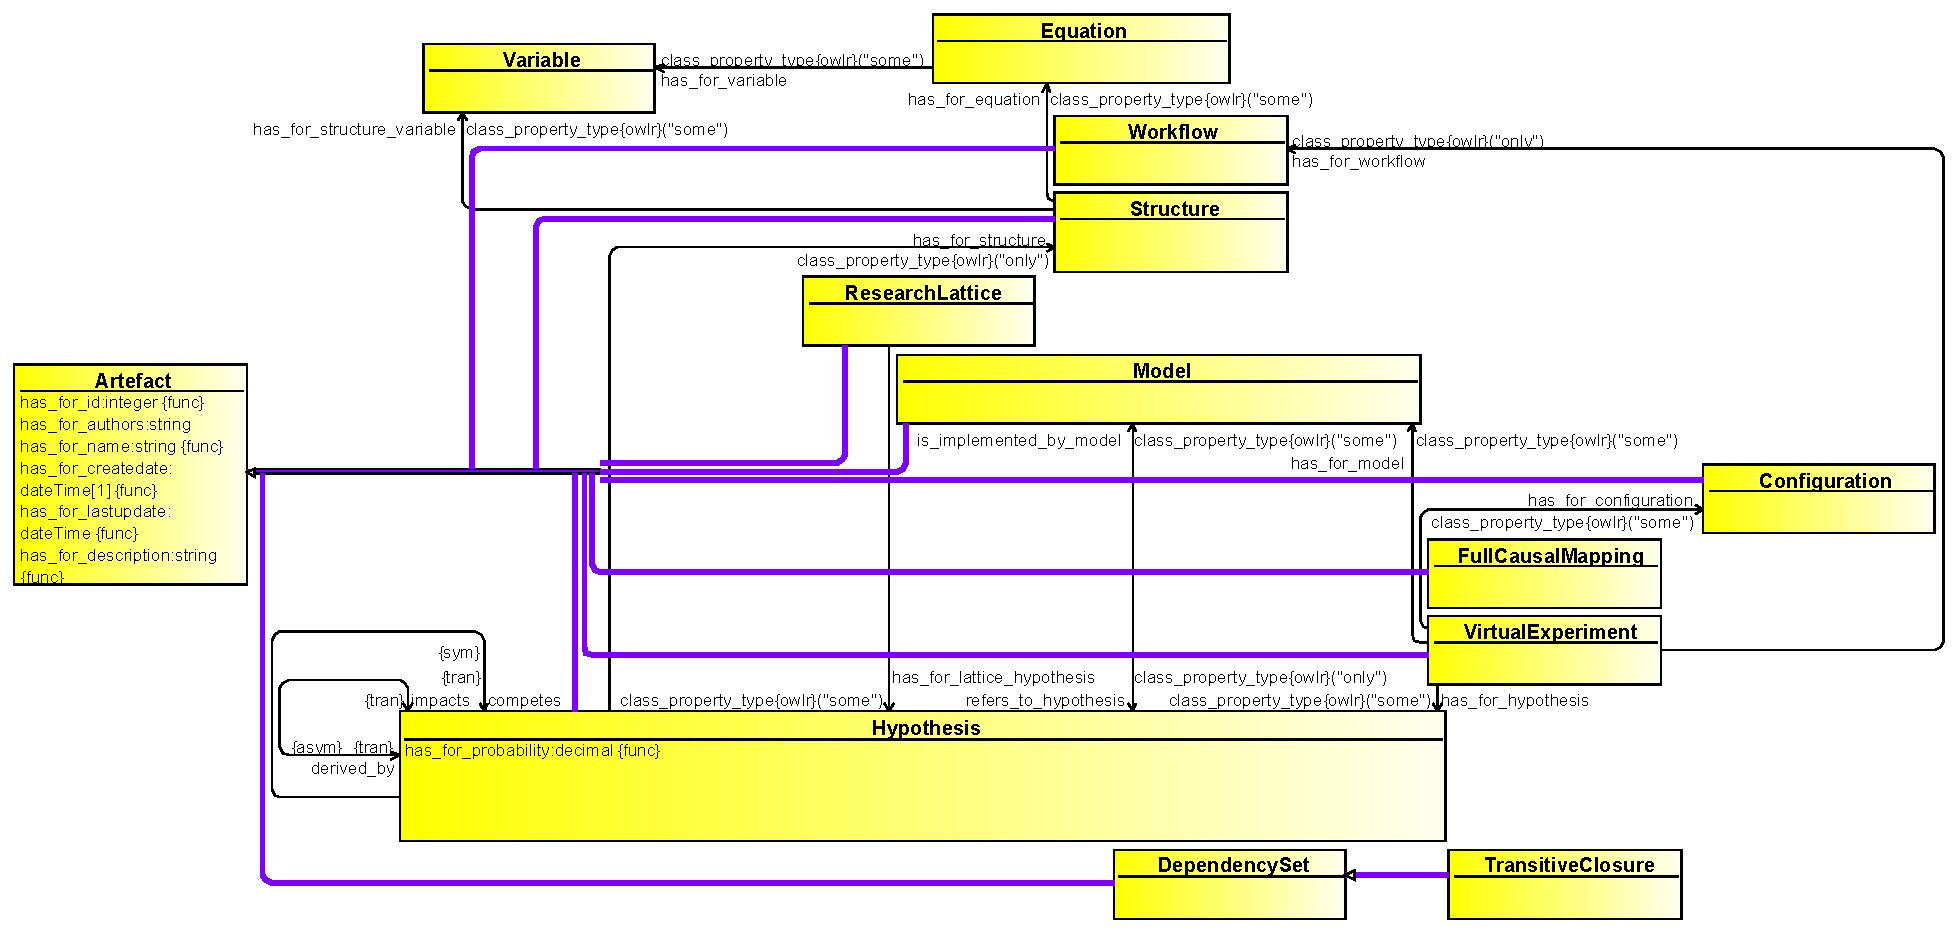
\includegraphics[width=\linewidth]{images/ve_schema2.pdf}
    \caption{Часть онтологии виртуального эксперимента.}\label{fig:ve_schema}
\end{figure}

Определен отдельный ядровой модуль, содержащий классы, соответствующие ключевым понятиям, используемым при работе 
с платформой "--- виртуальный эксперимент, гипотеза, модель, поток работ, конфигурация. Дополнительно определены 
вспомогательные классы переменной, уравнения, структуры, решетки гипотез, полного причинно-следственного отображения, 
множества зависимых переменных и их транзитивного замыкания. 

Модуль использует пакет OwlReady2 \cite{Lamy2017}, который позволяет программировать на Python, ориентированном на 
онтологии, и управлять онтологиями OWL2. Пакет поддерживает такие операции с онтологиями, как загрузка, сохранение, 
изменение, а также рассуждения. Это также позволяет комбинировать методы в Python с классами онтологии, как если бы 
они были объектами Python. Ниже приведен пример определений классов гипотез и моделей:

\begin{ListingEnv}[!h]% настройки floating аналогичны окружению figure
    \captiondelim{ } % разделитель идентификатора с номером от наименования
    \caption{Листинг}\label{lst:hwbeauty}
    % окружение учитывает пробелы и табуляции и применяет их в сответсвии с настройками
    \begin{lstlisting}[language={Python}]
    class has_for_name(Artefact >> str): pass
    class Artefact(Thing):
        is_a = [has_for_name.exactly(1)]
    ...
    class Hypothesis(Artefact): pass
    class Model(Artefact): pass
    class has_for_probability(Hypothesis >> float,
                            DataProperty,
                            FunctionalProperty): pass
    class is_implemented_by_model(Hypothesis >> Model): 
        class_property_type = ["some"]
    class refers_to_hypothesis(ObjectProperty):
        domain              = [Model]
        range               = [Hypothesis]
        inverse_property    = is_implemented_by_model
        class_property_type = ["only"]
    class competes(Hypothesis >> Hypothesis, 
        TransitiveProperty, SymmetricProperty): pass
    class derived_by(Hypothesis >> Hypothesis, 
        TransitiveProperty, AsymmetricProperty): pass
    class impacts(ObjectProperty, TransitiveProperty):
        domain              = [Hypothesis]
        range               = [Hypothesis]
        inverse_propert     = derived_by
    \end{lstlisting}
\end{ListingEnv}%

Гипотеза и модель являются подклассами класса артефактов с одним свойством name (среди прочих). Сюръективное 
отображение из гипотез в модели определяется с использованием свойств объекта 
\textit{is\textunderscore implemented\textunderscore by\textunderscore model} и 
\textit{refers\textunderscore to\textunderscore hypothesis}. Например, домен 
\textit{refers\textunderscore to\textunderscore hypothesis} "--- это модель, а диапазон "--- гипотеза. Отношение 
конкуренции определяется для гипотез как транзитивное и симметричное свойство. \textit{Derived\textunderscore by} 
определяется как транзитивное, но асимметричное свойство. Обратным к \textit{derived\textunderscore by} 
является отношение воздействий.

Гипотеза содержит класс структуры, структура содержит в себе множество уравнений и переменных, а также использует 
классы полного причинно-следственного отображения, множества зависимых переменных и их транзитивного замыкания. 
Решетка гипотез строится по множеству гипотез и потоку работ.




\section{Выводы по главе}\label{sect2_6}



\FloatBarrier
